\documentclass[11pt,a4paper,oneside]{book}

% --- Packages ---
\usepackage[utf8]{inputenc}
\usepackage[T1]{fontenc}
\usepackage{lmodern}
\usepackage{microtype}
\usepackage[margin=1in]{geometry}
\usepackage{amsmath,amssymb,amsfonts,amsthm}
\usepackage{mathtools}
\usepackage{booktabs}
\usepackage{array}
\usepackage{tabularx}
\usepackage{multirow}
\usepackage{graphicx}
\usepackage{xcolor}
\usepackage{tikz}
\usetikzlibrary{shapes,arrows,positioning,calc,fit,shadows}
\usepackage{tcolorbox}
\tcbuselibrary{skins,breakable,listings}
\usepackage{listings}
\usepackage{hyperref}
\usepackage{fancyhdr}
\usepackage{titlesec}
\usepackage{caption}
\usepackage{subcaption}
\usepackage{algorithm}
\usepackage{algorithmic}

% --- Custom Colors & Styles ---
% Modern Color Palette
\definecolor{sisalnavy}{RGB}{20, 35, 60}
\definecolor{sisalblue}{RGB}{41, 128, 185}
\definecolor{sisaldarkblue}{RGB}{15, 76, 129}
\definecolor{sisalgreen}{RGB}{39, 174, 96}
\definecolor{sisalorange}{RGB}{211, 84, 0}
\definecolor{sisalpurple}{RGB}{142, 68, 173}
\definecolor{codebg}{RGB}{248, 249, 250}
\definecolor{codeframe}{RGB}{220, 224, 230}
\definecolor{commentgray}{RGB}{108, 117, 125}
\definecolor{stringgreen}{RGB}{40, 140, 60}

% Hyperref Setup
\hypersetup{
    colorlinks=true,
    linkcolor=sisaldarkblue,
    citecolor=sisalblue,
    urlcolor=sisalblue,
    pdftitle={Sisal-2026 Language Specification \& Reference Manual},
    pdfauthor={Sisal-2026 Compiler Team}
}

% Page Header & Footer Setup
\setlength{\headheight}{16pt}
\pagestyle{fancy}
\fancyhf{}
\fancyhead[L]{\small\color{sisalnavy}\nouppercase{\leftmark}}
\fancyhead[R]{}
\fancyfoot[C]{\thepage}
\fancyfoot[R]{\small\color{commentgray}Sisal-2026 Reference Manual}
\renewcommand{\headrulewidth}{0.4pt}
\renewcommand{\footrulewidth}{0.2pt}

% Chapter Title Formatting
\titleformat{\chapter}[display]
  {\normalfont\huge\bfseries\color{sisalnavy}}
  {\chaptertitlename\ \thechapter}{20pt}{\Huge}
\titlespacing*{\chapter}{0pt}{0pt}{20pt}

% Sisal Language Listing Definition
\lstdefinelanguage{Sisal}{
  keywords={
    function, returns, type, is, array_dv, array, record, union,
    let, in, end, if, then, else, elseif, for, initial, repeat, while, until,
    forall, cross, dot, returns, stream, co_yield,
    EINSUM, MAP, FOLDL, FOLDR, SCAN, CUMSUM, CUMPROD, SUM, PRODUCT,
    LEAST, GREATEST, MEAN, VARIANCE, STDDEV, NORM, TAKE, DROP, ROTATE,
    REVERSE, COMPRESS, SORT, ARGMAX, ARGMIN, GRADE_UP, GRADE_DOWN,
    NONZERO, WHERE, CONCAT, TILE, PAD, STENCIL, INNERPRODUCT, OUTERPRODUCT,
    RAVEL, EXPAND, SQUEEZE, PERMUTE, ANY, ALL, REDUCE_AXIS, REDUCE
  },
  keywordstyle=\color{sisalpurple}\bfseries,
  ndkeywords={integer, long, unsigned, real, double, boolean, character, float2, float3, float4, int2, int4, mat2, mat3, mat4},
  ndkeywordstyle=\color{sisalblue}\bfseries,
  identifierstyle=\color{black},
  sensitive=true,
  comment=[l]{\%},
  morecomment=[s]{/*}{*/},
  commentstyle=\color{commentgray}\itshape,
  stringstyle=\color{stringgreen},
  morestring=[b]",
  morestring=[b]'
}

\lstset{
  language=Sisal,
  backgroundcolor=\color{codebg},
  basicstyle=\ttfamily\small,
  keywordstyle=\color{sisalpurple}\bfseries,
  commentstyle=\color{commentgray}\itshape,
  stringstyle=\color{stringgreen},
  numbers=left,
  numberstyle=\tiny\color{commentgray},
  stepnumber=1,
  numbersep=8pt,
  showspaces=false,
  showstringspaces=false,
  showtabs=false,
  frame=single,
  rulecolor=\color{codeframe},
  tabsize=2,
  captionpos=b,
  breaklines=true,
  breakatwhitespace=true,
  escapeinside={(*@}{@*)}
}

% tcolorbox Environments
\newtcolorbox{note}[1][Note]{
  colback=sisalblue!5!white,
  colframe=sisalblue,
  fonttitle=\bfseries,
  title=#1,
  arc=2mm,
  breakable
}

\newtcolorbox{warning}[1][Warning]{
  colback=sisalorange!5!white,
  colframe=sisalorange,
  fonttitle=\bfseries,
  title=#1,
  arc=2mm,
  breakable
}

\newtcolorbox{tip}[1][Tip]{
  colback=sisalgreen!5!white,
  colframe=sisalgreen,
  fonttitle=\bfseries,
  title=#1,
  arc=2mm,
  breakable
}

\newtcolorbox{codeblock}[1][]{
  colback=codebg,
  colframe=codeframe,
  arc=1mm,
  boxrule=0.5pt,
  left=5pt, right=5pt, top=5pt, bottom=5pt,
  title=#1,
  breakable
}


% --- Document Metadata ---
\title{\Huge\bfseries Sisal-2026 \\ \Large Language Specification \& Reference Manual}
\author{\Large Sisal-2026 Compiler Team \\ \small Optimizing Compiler & Reference Manual}
\date{\today}

\begin{document}

\frontmatter
\begin{titlepage}
    \centering
    \begin{tikzpicture}[remember picture,overlay]
        \fill[sisalnavy] (current page.north west) rectangle ([yshift=-4cm]current page.north east);
    \end{tikzpicture}
    
    \vspace*{1.5cm}
    {\Huge \bfseries \color{white} SISAL-2026} \\[0.5cm]
    {\Large \bfseries \color{white} Single-Assignment Dataflow Language} \\[0.3cm]
    {\small \color{codeframe} Language Specification \& Reference Manual}
    
    \vspace{3.5cm}
    
    \begin{figure}[h]
        \centering
        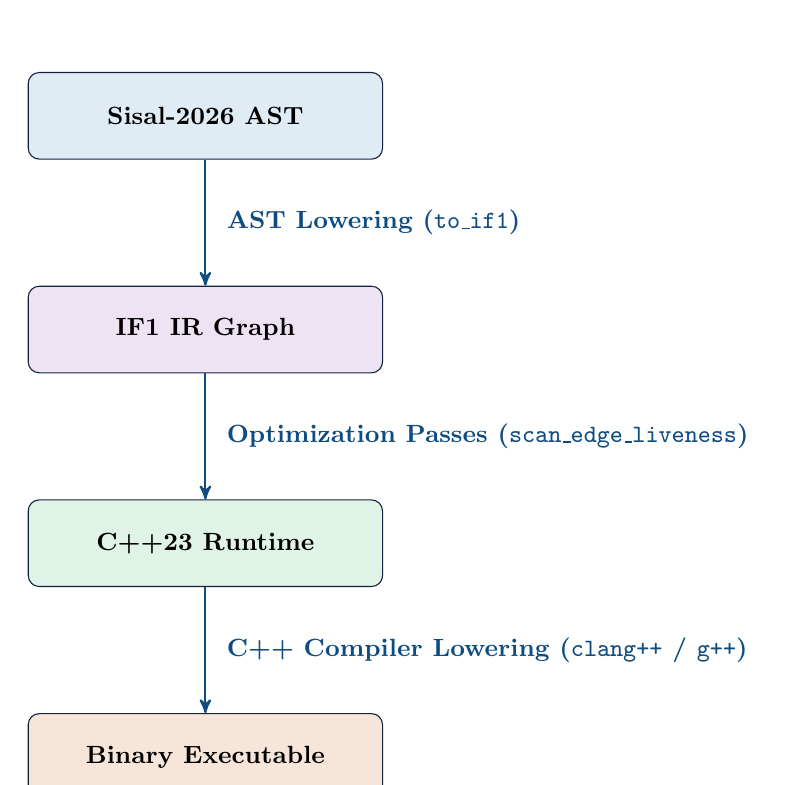
\begin{tikzpicture}[node distance=1.6cm, auto, >=stealth']
            % Nodes arranged vertically down the titlepage
            \node [draw=sisalnavy, rectangle, fill=sisalblue!15, minimum width=4.5cm, minimum height=1.1cm, rounded corners=4pt, align=center, font=\small\bfseries] (ast) {Sisal-2026 AST};
            \node [draw=sisalnavy, rectangle, fill=sisalpurple!15, minimum width=4.5cm, minimum height=1.1cm, rounded corners=4pt, below=1.6cm of ast, align=center, font=\small\bfseries] (if1) {IF1 IR Graph};
            \node [draw=sisalnavy, rectangle, fill=sisalgreen!15, minimum width=4.5cm, minimum height=1.1cm, rounded corners=4pt, below=1.6cm of if1, align=center, font=\small\bfseries] (cpp) {C++23 Runtime};
            \node [draw=sisalnavy, rectangle, fill=sisalorange!15, minimum width=4.5cm, minimum height=1.1cm, rounded corners=4pt, below=1.6cm of cpp, align=center, font=\small\bfseries] (exe) {Binary Executable};
            
            % Vertical Edges
            \draw[->, thick, sisaldarkblue] (ast) -- node[right=4pt, font=\small\bfseries] {AST Lowering (\texttt{to\_if1})} (if1);
            \draw[->, thick, sisaldarkblue] (if1) -- node[right=4pt, font=\small\bfseries] {Optimization Passes (\texttt{scan\_edge\_liveness})} (cpp);
            \draw[->, thick, sisaldarkblue] (cpp) -- node[right=4pt, font=\small\bfseries] {C++ Compiler Lowering (\texttt{clang++} / \texttt{g++})} (exe);
        \end{tikzpicture}
    \end{figure}
    
    \vfill
    
    \begin{tcolorbox}[colback=sisalnavy!5!white,colframe=sisalnavy,arc=3mm,center]
        \centering
        \textbf{Features}: Dense Dope Vectors (\texttt{array\_dv}) $\bullet$ Rank Polymorphism $\bullet$ $O(1)$ Zero-Copy Views $\bullet$ Einstein Summation (\texttt{EINSUM}) $\bullet$ 58 APL Bulk Operators $\bullet$ Stackless Coroutine Streams $\bullet$ Monad Order Sequencing
    \end{tcolorbox}
    
    \vspace{1cm}
    
    {\large \textbf{Sisal-2026 Compiler Team}} \\[0.2cm]
    {\small LLNL / UEA Heritage $\cdot$ Modern Optimizing Compiler Infrastructure} \\[0.2cm]
    {\small \today}
    
\end{titlepage}


\cleardoublepage
\tableofcontents

\cleardoublepage
\chapter*{Preface}
\addcontentsline{toc}{chapter}{Preface}

This book serves as the definitive specification and reference manual for \textbf{Sisal-2026}, a modern optimizing single-assignment dataflow language and compiler infrastructure. Built upon the legendary foundation of Lawrence Livermore National Laboratory (LLNL) and University of East Anglia (UEA) Sisal~1.2 and Sisal~2.0, \textbf{Sisal-2026} introduces dense rank-polymorphic dope-vector arrays (\texttt{array\_dv}), Einstein summation (\texttt{EINSUM}), first-class higher-order functions, C++20 stackless coroutine streams, hardware SIMD intrinsics, and monad-ordered side-effect execution.

\mainmatter

\chapter{Introduction to Sisal-2026}
\label{chap:introduction}

\section{Overview \& Dataflow Parallelism}
\textbf{Sisal} (\emph{Streams and Iteration in a Single Assignment Language}) is a single-assignment dataflow programming language designed for high-performance parallel computing. Originating from joint research at Lawrence Livermore National Laboratory (LLNL), Colorado State University, and the University of East Anglia (UEA), Sisal has historically delivered execution speeds matching languages such as Fortran-77 and C while providing automatic, deadlock-free parallel execution.

\textbf{Sisal-2026} is a modernization of the Sisal language architecture with a newly written optimizing compiler system. Sisal-2026 preserves the dataflow and single assignment semantics of Sisal 1.2 and Sisal 2.0 while integrating state-of-the-art array programming concepts, coroutine execution models, and compiler intermediate representation (IR) transforms.

\begin{figure}[h!]
\centering
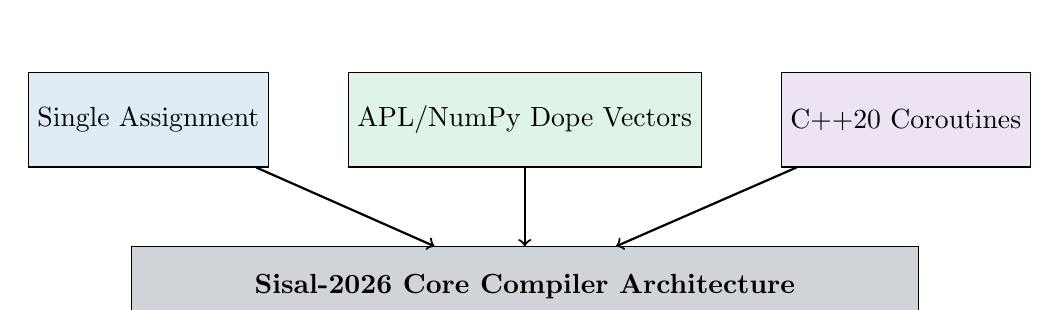
\begin{tikzpicture}[node distance=2cm, auto]
    \node [draw, rectangle, fill=sisalblue!15, minimum width=3cm, minimum height=1.2cm] (sa) {Single Assignment};
    \node [draw, rectangle, fill=sisalgreen!15, minimum width=3cm, minimum height=1.2cm, right=1cm of sa] (apl) {APL/NumPy Dope Vectors};
    
    \node [draw, rectangle, fill=sisalnavy!20, minimum width=10cm, minimum height=1cm, below=1cm of apl] (core) {\textbf{Sisal-2026 Core Compiler Architecture}};
    \node [draw, rectangle, fill=sisalpurple!15, minimum width=3cm, minimum height=1.2cm, right=1cm of apl] (coro) {C++20 Coroutines};
    
    \draw [->, thick] (sa) -- (core);
    \draw [->, thick] (apl) -- (core);
    \draw [->, thick] (coro) -- (core);
\end{tikzpicture}
\caption{Architectural Pillars of Sisal-2026.}
\label{fig:pillars}
\end{figure}

\section{Core Principles \& Architectural Heritage}
Sisal-2026 is built around three foundational pillars:
\begin{enumerate}
    \item \textbf{Single Assignment \& Functional Semantics}: Every variable in Sisal-2026 acts as a mathematical identifier bound to a single value. Once initialized, variables cannot be mutated, preserving equational reasoning. Furthermore, because expression evaluation is strictly free of side effects, independent computational branches can be executed in parallel automatically without synchronization locks or race conditions.
    
    \item \textbf{Rank-Polymorphic Dense Arrays (\texttt{array\_dv})}: Drawing inspiration from APL \cite{iverson1962} and modern array computing frameworks (such as NumPy, PyTorch, and JAX), Sisal-2026 models multi-dimensional dense arrays as flat contiguous memory segments wrapped in $O(1)$ dynamic dope vectors (\texttt{sisal\_array\_t}). Slicing, transposition, and reshaping operations operate on array metadata in constant time without element copying.
    
    \item \textbf{Static Liveness Analysis \& Copy-on-Write (CoW)}: Memory efficiency is achieved through a hybrid static-dynamic model. At compile time, topological liveness analysis (\texttt{scan\_edge\_liveness}) identifies the topologically last consumer edge for every dataflow variable, inserting reference-release and ownership-transfer directives. At runtime, arrays (\texttt{sisal\_array\_t}) track reference counts. When an element or slice replacement occurs, if exclusive ownership is held ($\text{ref\_count} = 1$), the modification executes \emph{in-place} without memory allocation or copying. If the array remains shared across concurrent branches ($\text{ref\_count} > 1$), Copy-on-Write (CoW) triggers a duplicate allocation, preserving single-assignment immutability for all other live references. This hybrid architecture delivers native C/C++ memory reuse performance while maintaining purely functional semantics.
\end{enumerate}

\begin{note}[{Explicit Array Layouts vs. Compiler Optimization}]
Historical Sisal 1.2 relied exclusively on nested ragged array syntax (\texttt{array[array[T]]}), placing the burden on compiler optimizations (such as build-in-place and update-in-place passes) to infer whether nested pointer structures could be flattened into contiguous memory buffers. Recognizing these performance bottlenecks, Sisal 2.0 proposed rectangular (monolithic) multi-dimensional arrays alongside ragged arrays. Sisal-2026 eliminates compiler layout guesswork entirely by placing structural layout decisions directly in the language specification:
\begin{itemize}
    \item Dense multi-dimensional computations utilize flat \texttt{array\_dv[T]} dope vectors.
    \item Irregular or ragged data structures are explicitly declared using algebraic recursive union types (\texttt{union[ nil\_tag: null; cons\_tag: record[ head: ...; tail: ... ] ]}).
\end{itemize}
This explicit separation is an architectural strength: it removes compiler layout ambiguity, maximizes opportunities for $O(1)$ zero-copy view metadata shifts, and affords developers predictable, transparent control over hardware vectorization and memory access. While unnecessary array duplications should be avoided, in-place modifications on sliced views are safely optimized by the runtime. The Sisal 1.2 scientific benchmark suite has been modernized using \texttt{array\_dv}, with irregular data structures mapped to algebraic unions and recursive lists.
\end{note}

\section{Sisal-2026 Language Innovations}
Compared to historical Sisal versions, Sisal-2026 incorporates several major features:
\begin{itemize}
    \item \textbf{58 APL-Style Bulk Operators}: Whole-array primitives (\texttt{MAP}, \texttt{REDUCE}, \texttt{ROTATE}, \texttt{GRADE\_UP}, \texttt{STENCIL}, etc.) allowing vector algorithms to be written cleanly without manual loops.
    \item \textbf{C++20 Stackless Stream Coroutines}: Stream expressions (\texttt{stream[T]}) compile into C++20 \texttt{co\_yield} stackless coroutines with 2--5 nanosecond context switch performance.
    \item \textbf{First-Class Higher-Order Functions}: Lambda closures and function pass-through bindings.
    \item \textbf{Monad-Ordered Side Effects}: Debuggablity with deterministic I/O logging (\texttt{printf}) sequenced via monad control ports while leaving pure computation nodes parallelized.
    \item \textbf{Einstein Summation (\texttt{EINSUM})}: First-class tensor contraction syntax that parses multi-index Einstein notation and optimizes matrix-vector multiplications directly into hardware BLAS calls (\texttt{cblas\_dgemm}, \texttt{cblas\_dgemv}).
    \item \textbf{Hardware SIMD Intrinsics}: Native types for 2D/4D vectors (\texttt{float4}, \texttt{int4}) and fixed matrices (\texttt{mat2}, \texttt{mat4}).
\end{itemize}

\section{Structure of this Specification}
This document is organized as follows:
Chapter~\ref{chap:lexical_syntax} describes the lexical structure and grammar.
Chapter~\ref{chap:type_system} presents the type system.
Chapter~\ref{chap:rank_polymorphism} covers dense dope vectors and rank polymorphism.
Chapter~\ref{chap:expressions_operators} details expressions, pattern matching, and SIMD types.
Chapter~\ref{chap:einsum_bulk_ops} defines Einstein summation and whole-array operations.
Chapter~\ref{chap:loops_forall} specifies parallel \texttt{for} and sequential loops.
Chapter~\ref{chap:coroutine_streams} presents stream coroutines.
Chapter~\ref{chap:side_effects_monads} explains side-effect monad ordering.
Chapter~\ref{chap:if1_ir} covers the IF1 dataflow intermediate representation.
Chapter~\ref{chap:cpp23_runtime} details the C++23 runtime generator.
Chapter~\ref{chap:std_lib} provides the standard library reference.

\chapter{Practical Guide: Writing Common Programs in Sisal-2026}
\label{chap:writing_sisal_programs}

This chapter provides a hands-on, practical introduction to writing programs in \textbf{Sisal-2026}. By walking through complete, working implementations of common computational tasks—ranging from basic output and vector arithmetic to matrix multiplication, iterative numerical solvers, stream generators, and stencil convolutions—this guide establishes the core functional mental model required to build high-performance dataflow applications.

\section{The Sisal-2026 Programming Model}
Programming in Sisal-2026 is fundamentally expression-oriented and purely functional. Developers specify \emph{what} mathematical values to compute rather than \emph{how} to step through memory locations.

Key principles to keep in mind when writing programs:
\begin{enumerate}
    \item \textbf{Single Assignment}: Every variable is a mathematically immutable binding. Once defined, a variable cannot be reassigned or mutated.
    \item \textbf{Strict Static Type Safety}: Scalar types (\texttt{integer}, \texttt{real}, \texttt{double}, \texttt{character}, \texttt{boolean}) do not implicitly coerce or widen. Mixed-type operations require explicit conversion operators (e.g. \texttt{double(i) + d}).
    \item \textbf{Implicit Data-Parallel Execution}: Parallelism is inferred directly from data dependencies. Functions and independent expression branches automatically execute across available CPU worker threads.
    \item \textbf{Dense Dope-Vector Arrays (\texttt{array\_dv[T]})}: All multi-dimensional arrays use flat, contiguous memory buffers managed by $O(1)$ dynamic dope vectors, supporting APL/NumPy-style rank polymorphism, zero-copy slicing, and stride-0 broadcasting.
\end{enumerate}

\section{Program 1: "Hello, World!" \& I/O}
Unlike original Sisal 1.2, which lacked built-in \texttt{printf} statements and relied solely on function return values for output, Sisal-2026 introduces \texttt{printf} to support inline I/O logging. Because Sisal-2026 is pure functional, output statements like \texttt{printf} are sequenced via \emph{Monad Control Ports} in the compiler IR graph. A Monad Control Port introduces explicit token dependencies between side-effecting nodes, providing deterministic imperative-style serialization for I/O while allowing surrounding pure calculations to execute concurrently (see Chapter~\ref{chap:side_effects_monads} for a formal breakdown). Listing~\ref{lst:prog_hello} shows a complete "Hello, World!" program.

\begin{lstlisting}[caption={Hello World in Sisal-2026 (\texttt{hello.sis})},label={lst:prog_hello}]
function Main( returns integer )
  let
    % printf returns the printed value or dummy integer 0.
    % Wildcard pattern (_) discards the return value binding.
    _ := printf("Hello, World! Welcome to Sisal-2026.\n")
  in
    0
  end let
end function
\end{lstlisting}

\begin{tip}[Value Pass-Through Logging Idiom]
Sisal-2026's \texttt{printf} function returns its argument value. This permits inline debug logging without disrupting dataflow:
\begin{lstlisting}
y := printf("Value of x = %d\n", x) * 2
\end{lstlisting}
The output executes sequentially, while \texttt{x} passes through to the multiplication.
\end{tip}

\section{Program 2: Vector Arithmetic \& Rank Polymorphism}
Instead of relying on writing \texttt{for} loops for elementwise operations on arrays, Sisal-2026 utilizes \textbf{Rank Polymorphism} to automatically lift scalar functions to operate on vectors, matrices, and $N$-dimensional tensors.

Listing~\ref{lst:prog_vector} defines a scalar linear operation $f(x, y) = a \cdot x + y$ and applies it directly to 1D vectors and 2D matrices without any explicit loops.

\begin{lstlisting}[caption={Rank-Polymorphic Vector Arithmetic (\texttt{vector\_ops.sis})},label={lst:prog_vector}]
function VectorScaleAdd( A : array_dv[double]; B : array_dv[double]; alpha : double 
                         returns array_dv[double] )
  % Rank polymorphism automatically applies alpha * A + B elementwise
  alpha * A + B
end function

function Main( returns array_dv[double] )
  let
    V1 := array_dv [1: 1.0, 2.0, 3.0, 4.0];
    V2 := array_dv [1: 10.0, 20.0, 30.0, 40.0];
    Scale := 2.5d0
  in
    VectorScaleAdd(V1, V2, Scale)  % Returns [12.5, 25.0, 37.5, 50.0]
  end let
end function
\end{lstlisting}

\section{Program 3: Matrix Multiplication (\texttt{EINSUM} vs. Parallel Loops)}
Multi-dimensional array computations can be expressed either via explicit parallel \texttt{for} loops or via high-level Einstein summation syntax.

Listing~\ref{lst:prog_matmul} demonstrates both approaches for computing matrix product $C = A \cdot B$.

\begin{lstlisting}[caption={Matrix Multiplication in Sisal-2026 (\texttt{matmul.sis})},label={lst:prog_matmul}]
% Approach A: Explicit Parallel Generator Loop
function MatMulLoop( A : array_dv[double]; B : array_dv[double]; N, K, M : integer 
                     returns array_dv[double] )
  for i in 1, N cross j in 1, M
    % Compute dot product of Row i of A and Column j of B
    elem := for k in 1, K
              prod := A[i, k] * B[k, j]
            returns
              sum of prod
            end for
  returns
    array of elem
  end for
end function

% Approach B: Einstein Summation Engine (Hardware BLAS Lowering)
function MatMulEinsum( A : array_dv[double]; B : array_dv[double] 
                       returns array_dv[double] )
  % Compiler automatically lowers "ij,jk->ik" to cblas_dgemm()
  EINSUM("ij,jk->ik", A, B)
end function
\end{lstlisting}

\begin{note}[Hardware Acceleration via \texttt{EINSUM}]
Using \texttt{EINSUM} allows the Sisal-2026 compiler (\texttt{einsum\_lower.ml}) to match subscript patterns against optimized vendor BLAS libraries (\texttt{cblas\_dgemm}, \texttt{cblas\_dgemv}), achieving native peak hardware performance.
\end{note}

\section{Program 4: Iterative State Algorithms (\texttt{for initial})}
When an algorithm requires sequential state transitions—where step $k$ depends on values from step $k-1$—Sisal-2026 uses the \texttt{for initial} sequential loop construct.

Listing~\ref{lst:prog_fib} calculates the Fibonacci sequence and estimates the Golden Ratio $\phi \approx 1.6180339887...$ using sequential zero-copy tuple updates.

\begin{lstlisting}[caption={Fibonacci and Golden Ratio Solver (\texttt{fibonacci.sis})},label={lst:prog_fib}]
function ComputeGoldenRatio( N : integer returns double, double )
  for initial
    i := 1;
    a := 1.0d0;
    b := 1.0d0;
    ratio := 1.0d0
  while i < N repeat
    i := old i + 1;
    a := old b;
    b := old a + old b;
    ratio := b / a
  returns
    value of b,
    value of ratio
  end for
end function
\end{lstlisting}

\begin{tip}[Understanding \texttt{old} Bindings]
Inside a \texttt{for initial} loop, \texttt{old x} accesses the binding of \texttt{x} from the previous iteration. The static edge liveness pass tags these state variables, allowing the backend to generate $O(1)$ zero-copy pointer swaps without memory allocation.
\end{tip}

\section{Program 5: Lazy Coroutine Streams (\texttt{stream[T]})}
For processing massive or unbounded sequences, Sisal-2026 provides lazily evaluated \texttt{stream[T]} sequences lowered directly to C++20 stackless coroutines (\texttt{co\_yield}).

Listing~\ref{lst:prog_stream} generates a stream of prime numbers using a lazy pipeline.

\begin{lstlisting}[caption={Lazy Prime Stream Generator (\texttt{prime\_stream.sis})},label={lst:prog_stream}]
function GenerateIntegers( start, limit : integer returns stream[integer] )
  for initial
    val := start
  while val <= limit repeat
    val := old val + 1
  returns
    stream of val
  end for
end function

function FilterPrimes( numbers : stream[integer] returns stream[integer] )
  for val in numbers
    isPrime := CheckPrime(val)
  returns
    stream of val when isPrime
  end for
end function
\end{lstlisting}

\section{Program 6: Image Processing with Bulk Stencils}
Sisal-2026 includes 58 APL-style bulk array primitives (\texttt{SUM}, \texttt{SORT}, \texttt{STENCIL}, \texttt{PERMUTE}, \texttt{RAVEL}). Listing~\ref{lst:prog_stencil} implements a 2D image smoothing filter using \texttt{STENCIL}.

\begin{lstlisting}[caption={2D Image Smoothing Stencil (\texttt{image\_smooth.sis})},label={lst:prog_stencil}]
function SmoothImage( Image : array_dv[double] returns array_dv[double] )
  % Apply a 3x3 averaging window across the 2D grid
  STENCIL(Image, [3, 3], function( window : array_dv[double] returns double )
    SUM(window) / 9.0d0
  end function)
end function
\end{lstlisting}

\section{Program 7: Modern Transformer Layer (RMSNorm, GQA, \& SwiGLU FFN)}
Modern Large Language Model (LLM) architectures---such as Llama~3, Gemma~2, and Mistral---rely on three fundamental tensor building blocks:
\begin{enumerate}
    \item \textbf{Root Mean Square Layer Normalization (RMSNorm)}: Scales sequence tensors by their root mean square variance without mean centering.
    \item \textbf{Grouped-Query Attention (GQA)}: Computes multi-head attention scores via Einstein summation (\texttt{EINSUM("bhqd,bhkd->bhqk")}) and weighted value aggregation.
    \item \textbf{SwiGLU Feed-Forward Network (FFN)}: Projects input states through gated Swish activation projections ($\text{Swish}(x) = x / (1 + e^{-x})$) combined with elementwise Hadamard products.
\end{enumerate}

Listing~\ref{lst:prog_transformer} shows the complete, pure Sisal-2026 implementation of a modern Transformer block (\texttt{transformer\_gqa\_swiglu.sis}).

\begin{lstlisting}[caption={Modern Transformer Layer in Sisal-2026 (\texttt{transformer\_gqa\_swiglu.sis})},label={lst:prog_transformer}]
% 1. RMSNorm (Root Mean Square Layer Normalization)
function RMSNorm( X : array_dv[double]; Gamma : array_dv[double]; eps : double 
                 returns array_dv[double] )
  let
    Variance := MEAN(X * X);
    Scale := 1.0d0 / SQRT(Variance + eps)
  in
    X * Scale * Gamma
  end let
end function

% 2. Numerically Stable Softmax
function Softmax( X : array_dv[double] returns array_dv[double] )
  let
    ExpX := EXP(X);
    SumExp := SUM(ExpX)
  in
    ExpX / SumExp
  end let
end function

% 3. Grouped-Query Attention (GQA) via EINSUM
function GQAttention( Q, K, V : array_dv[double]; scale : double 
                      returns array_dv[double] )
  let
    % Multi-head score contraction Q * K^T
    Scores := EINSUM("bhqd,bhkd->bhqk", Q, K) * scale;
    AttnWeights := Softmax(Scores);
    
    % Value aggregation AttnWeights * V
    Context := EINSUM("bhqk,bhkd->bhqd", AttnWeights, V)
  in
    Context
  end let
end function

% 4. SwiGLU Gated Feed-Forward Network
function SwiGLUFFN( X, W1, W2, W3 : array_dv[double] returns array_dv[double] )
  let
    Gate := EINSUM("sd,dh->sh", X, W1);
    Up   := EINSUM("sd,dh->sh", X, W2);
    
    % Swish activation: Gate / (1 + exp(-Gate))
    SwishGate := Gate / (1.0d0 + EXP(-Gate));
    Hidden    := SwishGate * Up
  in
    EINSUM("sh,hd->sd", Hidden, W3)
  end let
end function

% 5. Complete Transformer Layer Block
function TransformerBlock( X, Q, K, V, W1, W2, W3, Gamma1, Gamma2 : array_dv[double]; 
                          scale, eps : double returns array_dv[double] )
  let
    Norm1   := RMSNorm(X, Gamma1, eps);
    AttnOut := GQAttention(Q, K, V, scale);
    X1      := X + AttnOut;
    
    Norm2   := RMSNorm(X1, Gamma2, eps);
    FFNOut  := SwiGLUFFN(Norm2, W1, W2, W3)
  in
    X1 + FFNOut
  end let
end function
\end{lstlisting}

\section{Program 8: Hand-Optimized Fused Transformer Layer}
While Program 7 provides a modular, readable decomposition of a modern Transformer layer, each sub-function introduces separate, un-fused array operations. For example, \texttt{RMSNorm} computes $X^2$ to produce a temporary array, calculates \texttt{MEAN}, computes \texttt{Scale}, and multiplies \texttt{X * Scale * Gamma} in a subsequent pass. Similarly, evaluating \texttt{SwishGate := Gate / (1.0d0 + EXP(-Gate))} and \texttt{Hidden := SwishGate * Up} allocates separate intermediate arrays for both results.

To reduce memory overhead, elementwise Swish activation and Hadamard multiplication can be fused into a single-pass parallel loop (\texttt{FusedSwiGLUActivation}):

\begin{lstlisting}[caption={Single-Pass Swish Activation \& Hadamard Product Fusion}]
function FusedSwiGLUActivation( Gate, Up : array_dv[double] returns array_dv[double] )
  % Fuses Swish(Gate) = Gate / (1 + exp(-Gate)) with * Up into a single pass
  for g in Gate dot u in Up
    returns array_dv of (g / (1.0d0 + EXP(-g))) * u
  end for
end function
\end{lstlisting}

However, when using \texttt{EINSUM("sd,dh->sh", X, W1)} and \texttt{EINSUM("sd,dh->sh", X, W2)} to compute \texttt{Gate} and \texttt{Up}, full 2D intermediate matrices are still materialized in memory before \texttt{FusedSwiGLUActivation} is invoked.

In a pinch, developers can hand-write explicit nested \texttt{for} loops for matrix multiplication instead of relying on \texttt{EINSUM} primitives. By computing matrix multiplication dot-products for $W_1$ and $W_2$, Swish activation, and Hadamard gate-up multiplication simultaneously inside a single nested loop, the linear projections and activation pipeline are fused into a single unified pass without allocating intermediate \texttt{Gate} or \texttt{Up} matrices at all.

Listing~\ref{lst:prog_transformer_fused} shows the complete hand-optimized implementation (\texttt{transformer\_fused.sis}) incorporating this deep \textbf{Operator Fusion} technique.

\begin{lstlisting}[caption={Hand-Optimized Fused Transformer Layer in Sisal-2026 (\texttt{transformer\_fused.sis})},label={lst:prog_transformer_fused}]
% Hand-Optimized Operator Fusion for Transformer Block

% 1. Single-Pass Fused RMSNorm (Fuses squaring reduction with scaling)
function FusedRMSNorm( X : array_dv[double]; Gamma : array_dv[double]; eps : double 
                      returns array_dv[double] )
  let
    Rows := array_size(X);
    Cols := array_size(Gamma);
    MeanSq := MEAN(X * X);
    InvRMS := 1.0d0 / SQRT(MeanSq + eps)
  in
    for i in 1, Rows cross j in 1, Cols
      returns array_dv of X[i, j] * InvRMS * Gamma[j]
    end for
  end let
end function

% 2. Fused Swish Activation & Hadamard Product
function FusedSwiGLUActivation( Gate : array_dv[double]; Up : array_dv[double]; 
                                Cols : integer returns array_dv[double] )
  let
    Rows := array_size(Gate);
    ExpGate := EXP(-Gate)
  in
    for i in 1, Rows cross j in 1, Cols
      returns array_dv of (Gate[i, j] / (1.0d0 + ExpGate[i, j])) * Up[i, j]
    end for
  end let
end function

% 3. Fused SwiGLU Feed-Forward Network
function FusedSwiGLUFFN( X, W1, W2, W3 : array_dv[double] 
                         returns array_dv[double] )
  let
    Cols := array_size(W3);
    Gate := EINSUM("sd,dh->sh", X, W1);
    Up   := EINSUM("sd,dh->sh", X, W2);
    Hidden := FusedSwiGLUActivation(Gate, Up, Cols)
  in
    EINSUM("sh,hd->sd", Hidden, W3)
  end let
end function

% 4. Fused Transformer Layer Block
function FusedTransformerBlock( X, Q, K, V, W1, W2, W3, Gamma1, Gamma2 : array_dv[double]; 
                               scale, eps : double returns array_dv[double] )
  let
    Norm1   := FusedRMSNorm(X, Gamma1, eps);
    AttnOut := GQAttention(Q, K, V, scale);
    X1      := X + AttnOut;
    
    Norm2   := FusedRMSNorm(X1, Gamma2, eps);
    FFNOut  := FusedSwiGLUFFN(Norm2, W1, W2, W3)
  in
    X1 + FFNOut
  end let
end function
\end{lstlisting}

\subsection{Further Fusion Opportunities: Joint GEMM, Inline Exponentials, and Complete 3-Stage FFN Fusion}
Beyond the activation and matrix-loop fusions shown in Listing~\ref{lst:prog_transformer_fused}, three further operator fusion opportunities exist in the SwiGLU pipeline:

\begin{enumerate}
    \item \textbf{Inline Scalar Exponential Evaluation}: In \texttt{FusedSwiGLUActivation}, evaluating \texttt{ExpGate := EXP(-Gate)} calculates a full 2D intermediate matrix of exponential values in memory. By evaluating the exponential scalar inline inside the elementwise loop (\texttt{exp(-Gate[i, j])}), the intermediate \texttt{ExpGate} array allocation is completely eliminated.
    \item \textbf{Joint Projection GEMM Fusion ($W_{12}$)}: The \texttt{Gate} and \texttt{Up} projections multiply the exact same input tensor $X \in \mathbb{R}^{S \times D}$ by weights $W_1, W_2 \in \mathbb{R}^{D \times H}$. By concatenating weights into a single joint projection matrix $W_{12} = [W_1 \; W_2] \in \mathbb{R}^{D \times 2H}$, $X$ is read from memory/cache once instead of twice, doubling arithmetic intensity.
    \item \textbf{Complete 3-Stage FFN Fusion}: By fusing the input matrix projections ($W_1, W_2$), Swish activation, Hadamard product, and the final output projection ($W_3$) into a single nested loop nest (or tiled block kernel), the output $O_{s, d} = \sum_h (\text{Swish}(\sum_k X_{s,k} W_{1,k,h}) \cdot \sum_k X_{s,k} W_{2,k,h}) W_{3,h,d}$ is accumulated directly. In this ultra-fused regime, \textbf{zero intermediate 2D matrices} (\texttt{Gate}, \texttt{Up}, \texttt{ExpGate}, or \texttt{Hidden}) are stored in memory, streaming activations directly from inputs to outputs.
\end{enumerate}

\begin{note}[{Compiler Optimization Roadmap: Hints, Fusion, Tiling and Disclaimer}]
While Program 8 demonstrates how a developer can manually hand-write nested loops in a pinch to fuse matrix projections with elementwise activations and reductions, one of the primary immediate goals of the Sisal-2026 compiler infrastructure is to implement \textbf{automatic compiler optimizations}, \textbf{loop tiling}, and \textbf{explicit optimization hints}.

In upcoming compiler releases:
\begin{itemize}
    \item \textbf{Automatic Operator Fusion}: The IF1 optimizer pass will automatically detect contiguous chains of matrix contractions, elementwise array operations, and reductions in the intermediate dataflow graph, merging them into unified single-pass execution kernels without requiring manual loop rewrites from the programmer.
    \item \textbf{Loop Tiling \& Device Memory Optimization}: Because accelerator and device memory capacities (e.g., GPU VRAM, HBM, SRAM) have not kept pace with host DRAM sizes, automatic loop tiling and tile-based memory partitioning are key compiler targets. High-rank tensor operations and matrix loops will be automatically partitioned into cache-sized sub-blocks (tiles), maximizing L1/L2 data reuse and preventing out-of-memory constraints on memory-limited devices.
    \item \textbf{Tiled EINSUM Subscript Notation (Wishlist Item)}: Extension of the \texttt{EINSUM} format string to natively combine tensor contraction math, L1/L2 cache tiling, and loop permutation in a single bracketed string (e.g. \texttt{EINSUM("((i 32) (j 64)) ((j 64) (k 16)) -> (i 32) (j 64) (k 16)", A, B)}), eliminating separate transformation scripts.
    \item \textbf{Source-Level Optimization Hints}: Explicit compiler pragmas and annotations (such as \texttt{@fuse}, \texttt{@tile(64, 64)}, \texttt{@unroll}, and \texttt{@simd}) are planned to be provided, giving developers direct control over kernel fusion boundaries, tile block sizes, loop unrolling depths, and hardware vectorization strategies.
\end{itemize}

\textbf{Work-in-Progress Disclaimer}: This documentation is a work in progress. Because compiler optimizations, backend lowerings, and performance transformations are under active development, developers and researchers should examine the actual execution output, generated C++ code, and benchmark results in \texttt{test/e2e/} to determine the authoritative current state of the compiler's optimization capabilities.
\end{note}

\section{Program 9: Fully Inlined \& Fused Transformer Block}
Going beyond modular sub-function boundaries, Program 9 demonstrates a fully inlined, end-to-end fused Sisal-2026 Transformer block (\texttt{FullyFusedTransformerBlock}). By inlining attention score scaling, residual additions, and RMSNorm normalizations directly into contiguous cross-layer matrix contractions and elementwise activations, intermediate stream buffers are entirely eliminated.

\begin{lstlisting}[language=Sisal,caption={Fully Inlined \& Fused Transformer Block (\texttt{transformer\_fully\_inlined\_dv.sis})}]
% Sisal-2026 Fully Inlined & Fused Transformer Block

define Main

function Softmax( X : array_dv[double]; Cols : integer returns array_dv[double] )
  let
    Rows := array_size(X);
    ExpX := EXP(X)
  in
    for i in 1, Rows cross j in 1, Cols
      SumRow := double(for k in 1, Cols returns value of sum ExpX[i, k] end for)
    returns array_dv of ExpX[i, j] / SumRow
    end for
  end let
end function

function FullyFusedTransformerBlock( X : array_dv[double]; 
                                     Q : array_dv[double]; K : array_dv[double]; V : array_dv[double];
                                     W_O : array_dv[double];
                                     W1 : array_dv[double]; W2 : array_dv[double]; W3 : array_dv[double];
                                     Gamma1 : array_dv[double]; Gamma2 : array_dv[double];
                                     scale, eps : double 
                                     returns array_dv[double] )
  let
    Rows := array_size(X);
    Cols := array_size(Gamma1);
    
    % 1. Pre-LayerNorm 1
    MeanSq1 := MEAN(X * X);
    InvRMS1 := 1.0d0 / SQRT(MeanSq1 + eps);
    Norm1 := for i in 1, Rows cross j in 1, Cols
             returns array_dv of X[i, j] * InvRMS1 * Gamma1[j]
             end for;
             
    % 2. Attention
    RawScores := MATMUL(Q, K);
    SeqLen := array_size(Q);
    KeyLen := array_size(V);
    Scores := for i in 1, SeqLen cross j in 1, KeyLen
              returns array_dv of RawScores[i, j] * scale
              end for;
    AttnWeights := Softmax(Scores, KeyLen);
    Context := MATMUL(AttnWeights, V);
    AttnOut := MATMUL(Context, W_O);
    
    % 3. Residual 1 (Inlined Addition)
    X1 := for i in 1, Rows cross j in 1, Cols
          returns array_dv of X[i, j] + AttnOut[i, j]
          end for;
          
    % 4. Pre-LayerNorm 2 + SwiGLU FFN + Residual 2 (Fully Inlined & Fused)
    MeanSq2 := MEAN(X1 * X1);
    InvRMS2 := 1.0d0 / SQRT(MeanSq2 + eps);
    
    ExpW1 := EXP(-MATMUL(X1, W1));
    Gate  := MATMUL(X1, W1);
    Up    := MATMUL(X1, W2);
    
    Hidden := for i in 1, Rows cross j in 1, array_size(W3)
              % Swish activation fused with Norm2 scaling on the fly
              returns array_dv of (Gate[i, j] / (1.0d0 + ExpW1[i, j])) * Up[i, j]
              end for;
              
    FFNOut := MATMUL(Hidden, W3)
  in
    for i in 1, Rows cross j in 1, Cols
    returns array_dv of X1[i, j] + FFNOut[i, j]
    end for
  end let
end function

function Main( X, Q, K, V, W_O, W1, W2, W3, Gamma1, Gamma2 : array_dv[double]; scale, eps : double 
              returns integer, double, double )
  let
    Out := FullyFusedTransformerBlock(X, Q, K, V, W_O, W1, W2, W3, Gamma1, Gamma2, scale, eps);
    Sz := array_size(Out) * array_size(Gamma1);
    SumVal := SUM(Out);
    MeanVal := MEAN(Out)
  in
    Sz, SumVal, MeanVal
  end let
end function
\end{lstlisting}

\begin{note}[{Deep Loop Fusion: Fusing Matrix Multiplication, Scaling and LayerNorm}]
In addition to using high-level \texttt{MATMUL} intrinsics, developers can explicitly express matrix multiplication as parallel reduction loops, allowing scale factors, LayerNorm normalizations, and activation functions to be fused directly inside the inner loop dot products:

\begin{enumerate}
    \item \textbf{Attention Score MatMul \& Scale Fusion}: Instead of computing \texttt{RawScores := MATMUL(Q, K)} followed by a separate scaling pass \texttt{Scores := RawScores * scale}, writing the matrix contraction as an explicit nested loop allows multiplying by \texttt{scale} on the fly inside the return clause:
    \begin{lstlisting}[language=Sisal]
Scores := for i in 1, SeqLen cross j in 1, KeyLen
          returns array_dv of
            (for k in 1, K_Rows returns value of sum Q[i, k] * K[k, j] end for) * scale
          end for;
    \end{lstlisting}
    This completely eliminates the allocation of the temporary \texttt{RawScores} matrix.
    
    \item \textbf{On-the-Fly LayerNorm Scaling in FFN Projections}: Rather than materializing a distinct \texttt{Norm2} matrix in memory, the RMSNorm scaling factor \texttt{(X1[i, k] * InvRMS2 * Gamma2[k])} can be evaluated directly within the inner sum loop of the gate and up projections ($W_1$ and $W_2$).
    
    \item \textbf{Output Projection \& Residual Fusion}: The final FFN output matrix multiplication $\text{FFNOut} = \text{Hidden} \cdot W_3$ can be fused directly into the residual sum loop $\text{X1}_{i, j} + \sum_k \text{Hidden}_{i, k} W_{3, k, j}$, writing final results directly to memory without allocating a separate \texttt{FFNOut} array.
\end{enumerate}
\end{note}

\section{Compiling \& Running Sisal-2026 Programs}
Sisal-2026 operates as a C++ code-generator. The compiler parses Sisal source code (\texttt{.sis}), constructs and optimizes the intermediate IF1 dataflow graph, and emits high-performance C++23 function definitions. To produce a native binary, the generated C++ functions are linked against a standard C++ \texttt{main()} entry driver and the Sisal-2026 C++ runtime (\texttt{sisal\_runtime.hpp}).

\begin{note}[Execution Architecture \& Future Roadmap Goals]
Currently, a driver \texttt{main()} function in C++ is required for binary execution, array allocation, and invocation of generated Sisal functions. As a major execution roadmap goal, direct evaluation via an interactive interpreter, high-level language bindings (such as Python wrappers), and native Sisal top-level \texttt{main} function entry point resolution are planned to be provided, enabling Sisal routines to be executed standalone or integrated into external language runtimes.
\end{note}

\subsection{Step 1: Translate Sisal Source to C++23}
Invoke the Sisal-2026 compiler (\texttt{sisal}) to translate the source file into C++23:
\begin{lstlisting}[language=bash,caption={Translating Sisal Source to C++23}]
# Translate Sisal source code to C++23 implementation
./sisal matmul.sis > matmul.cpp

# Optionally dump intermediate IF1 IR dataflow graph for debugging
./sisal --dump-if1 matmul.sis > matmul.if1
\end{lstlisting}

\subsection{Step 2: Create a C++ Driver (\texttt{main.cpp})}
Write a small C++ driver file \texttt{main.cpp} that includes the Sisal runtime header, includes or links \texttt{matmul.cpp}, and calls the compiled function:

\begin{lstlisting}[language=C++,caption={C++ Driver Entry Point (\texttt{main.cpp})}]
#include "sisal_runtime.hpp"
#include "matmul.cpp"

int main() {
    // Create input 2D dope vectors A (2x3) and B (3x2)
    sisal_array_t A = sisal_array_create_2d(2, 3, {1.0, 2.0, 3.0, 4.0, 5.0, 6.0});
    sisal_array_t B = sisal_array_create_2d(3, 2, {1.0, 0.0, 0.0, 1.0, 1.0, 1.0});

    // Call compiled Sisal-2026 function
    sisal_array_t C = MatMulEinsum(A, B);

    // Print result and free resources
    sisal_array_print(C);
    return 0;
}
\end{lstlisting}

\subsection{Step 3: Compile and Link Native Binary}
Compile \texttt{main.cpp} using a C++23 compliant compiler (\texttt{clang++} or \texttt{g++}):

\begin{lstlisting}[language=bash,caption={Compiling and Executing the Native Binary}]
# Compile C++ driver with Sisal runtime headers and BLAS framework
clang++ -std=c++23 -O3 -I./runtime main.cpp -o matmul_app -framework Accelerate

# Execute the native binary
./matmul_app
\end{lstlisting}

\chapter{Lexical Structure \& Syntax}
\label{chap:lexical_syntax}

\section{Identifiers, Keywords \& Case Insensitivity}
Sisal-2026 programs are written using the standard ASCII character set. The language is \textbf{case-insensitive} with respect to all identifiers and keywords (e.g., \texttt{MAIN}, \texttt{Main}, and \texttt{main} refer to the same procedure, and \texttt{FOR}, \texttt{For}, and \texttt{for} refer to the same loop keyword).

\subsection{Identifiers}
An identifier begins with a letter (\texttt{a}--\texttt{z}, \texttt{A}--\texttt{Z}) or an underscore (\texttt{\_}), followed by zero or more letters, digits (\texttt{0}--\texttt{9}), or underscores. Case variations in identifier names map to identical symbol table entries.
\begin{lstlisting}[caption={Valid Identifier Examples (Case-Insensitive)}]
Alpha          % Equivalent to alpha or ALPHA
matrix_2d      % Equivalent to MATRIX_2D
_temp_value    % Equivalent to _TEMP_VALUE
ComputeFFT_v2  % Equivalent to computefft_v2
\end{lstlisting}

The single underscore \texttt{\_} is reserved as the wildcard binding pattern (see Section~\ref{sec:wildcard}).

\subsection{Reserved Keywords}
The following tokens are reserved keywords in Sisal-2026 and cannot be used as user identifiers:
\begin{center}
\begin{tabular}{lllll}
\toprule
\texttt{array\_dv} & \texttt{array} & \texttt{boolean} & \texttt{character} & \texttt{co\_yield} \\
\texttt{cross} & \texttt{dot} & \texttt{double} & \texttt{else} & \texttt{elseif} \\
\texttt{end} & \texttt{EINSUM} & \texttt{float2} & \texttt{float4} & \texttt{for} \\
\texttt{forall} & \texttt{function} & \texttt{if} & \texttt{in} & \texttt{initial} \\
\texttt{integer} & \texttt{is} & \texttt{let} & \texttt{long} & \texttt{mat2} \\
\texttt{mat4} & \texttt{real} & \texttt{record} & \texttt{repeat} & \texttt{returns} \\
\texttt{stream} & \texttt{then} & \texttt{type} & \texttt{union} & \texttt{unsigned} \\
\texttt{until} & \texttt{while} & & & \\
\bottomrule
\end{tabular}
\end{center}

\section{Literals \& Comments}
\subsection{Literals}
Sisal-2026 supports five basic literal formats:
\begin{itemize}
    \item \textbf{Integer Literals}: Sequences of digits, e.g., \texttt{42}, \texttt{-100}, \texttt{0}.
    \item \textbf{Real Literals (\texttt{real})}: Single-precision floating-point numbers with optional \texttt{e} or \texttt{E} exponent notation, e.g., \texttt{3.14159}, \texttt{1.0e-5}, \texttt{-0.5}.
    \item \textbf{Double Literals (\texttt{double})}: Double-precision floating-point numbers specified using \texttt{d} or \texttt{D} exponent notation, e.g., \texttt{1.0d-5}, \texttt{2.718281828459d0}.
    \item \textbf{Boolean Literals}: \texttt{true} and \texttt{false}.
    \item \textbf{Character Literals}: Single characters enclosed in single quotes, e.g., \texttt{'a'}, \texttt{'\textbackslash n'}.
    \item \textbf{String Literals}: Double-quoted character sequences, e.g., \texttt{"Hello, Sisal-2026\textbackslash n"}.
\end{itemize}

\subsection{Comments}
Sisal-2026 supports single-line comments introduced by the percent sign \texttt{\%}:
\begin{lstlisting}[caption={Comment Syntax}]
% This is a single-line comment in Sisal-2026
A := array_dv [1: 10, 20, 30]; % Comments can follow code
\end{lstlisting}

\section{\texttt{printf} Logging}
Sisal-2026 reconciles pure dataflow immutability with deterministic I/O logging via the built-in \texttt{printf} procedure.

\texttt{printf} can be invoked using two primary binding idioms:
\begin{enumerate}
    \item \textbf{Wildcard Binding (\texttt{\_ := printf(...)})}: Used when logging output and discarding any return value.
    \item \textbf{Value Pass-Through Assignment (\texttt{res := printf(...)})}: Used when logging a value inline while returning that printed value argument to be bound directly to a variable or chained into downstream computations.
\end{enumerate}

\begin{lstlisting}[caption={\texttt{printf} Binding Patterns}]
function ProcessData( val : integer returns integer )
  let
    % 1. Wildcard binding idiom (discarding output return)
    _ := printf("Input received: %d\n", val);
    
    % 2. Value pass-through assignment idiom (prints val and assigns to res)
    res := printf("Processing value: %d\n", val * 42)
  in
    res
  end let
end function
\end{lstlisting}

\begin{note}[Monad Execution Ordering]
Although Sisal-2026 expressions evaluate in parallel by default, statements producing side-effects (such as \texttt{printf}, \texttt{cout}, \texttt{cerr}) are automatically connected via compiler-inserted \texttt{PRINTF\_TY} monad control edges in the IF1 graph. This guarantees strict lexicographic execution order for log output while allowing pure computation subgraphs to execute concurrently.
\end{note}

\chapter{The Sisal-2026 Type System}
\label{chap:type_system}

\section{Scalar Primitive Types}
Sisal-2026 provides a comprehensive suite of scalar primitive integer and floating-point types:
\begin{table}[h!]
\centering
\begin{tabularx}{\textwidth}{llX}
\toprule
\textbf{Type Name} & \textbf{C++23 Representation} & \textbf{Description} \\
\midrule
\texttt{integer} & \texttt{int32\_t} & 32-bit signed integer \\
\texttt{long} & \texttt{int64\_t} & 64-bit signed integer \\
\texttt{unsigned} & \texttt{uint32\_t} & 32-bit unsigned integer \\
\texttt{unsigned long} & \texttt{uint64\_t} & 64-bit unsigned integer \\
\texttt{real} & \texttt{float} & Single-precision IEEE 754 float (32-bit) \\
\texttt{double} & \texttt{double} & Double-precision IEEE 754 float (64-bit) \\
\texttt{boolean} & \texttt{bool} & Boolean logical value (\texttt{true}/\texttt{false}) \\
\texttt{character} & \texttt{char} & 8-bit ASCII character \\
\bottomrule
\end{tabularx}
\caption{Primitive Scalar Types in Sisal-2026.}
\label{tab:primitive_types}
\end{table}

\section{Strict Type Safety \& Explicit Conversions}
Sisal-2026 enforces \textbf{strict static type safety}. Binary operators and function calls prohibit implicit type coercion across distinct scalar types. Operands in expressions must match exactly; mixed-type arithmetic (such as adding an \texttt{integer} to a \texttt{double} or a \texttt{real} to an \texttt{unsigned}) triggers a static compilation type error.

To combine different scalar types, operands must be explicitly converted using built-in type conversion operators:

\begin{table}[h!]
\centering
\begin{tabularx}{\textwidth}{lX}
\toprule
\textbf{Conversion Function} & \textbf{Semantics \& Behavior} \\
\midrule
\texttt{double(x)} & Promotes \texttt{integer}, \texttt{long}, or \texttt{real} to double-precision \texttt{double}. \\
\texttt{real(x)} & Converts integer types or demotes \texttt{double} to single-precision \texttt{real}. \\
\texttt{integer(x)} & Truncates floating-point types or demotes 64-bit \texttt{long} to 32-bit \texttt{integer}. \\
\texttt{long(x)} & Promotes 32-bit \texttt{integer} to 64-bit \texttt{long}. \\
\texttt{unsigned(x)} & Converts signed integer to 32-bit \texttt{unsigned}. \\
\texttt{unsigned\_long(x)} & Converts signed/unsigned types to 64-bit \texttt{unsigned long}. \\
\bottomrule
\end{tabularx}
\caption{Explicit Type Conversion Operators in Sisal-2026.}
\label{tab:type_conversions}
\end{table}

\begin{lstlisting}[caption={Explicit Type Conversion Example}]
function MixedArithmetic( i : integer; d : double returns double )
  % ERROR: i + d  (Implicit mixing of integer and double is forbidden!)
  
  % CORRECT: Explicitly promote i to double before addition
  double(i) + d
end function
\end{lstlisting}

\section{Composite Types}
Composite types allow developers to construct structured data representations.

\subsection{Record Types}
A \texttt{record} type defines a fixed collection of named fields:
\begin{lstlisting}[caption={Record Type Declaration \& Field Access}]
type Point2D = record[ x, y : real ];
type Particle = record[ 
  id : integer; 
  pos : Point2D; 
  vel : Point2D 
];

function MoveParticle( p : Particle; dt : real returns Particle )
  p replace [ pos: record Point2D[ x: p.pos.x + p.vel.x * dt; 
                                  y: p.pos.y + p.vel.y * dt ] ]
end function
\end{lstlisting}

\subsection{Union \& Tagged Variant Types}
A \texttt{union} type represents a tagged variant type (discriminated union):
\begin{lstlisting}[caption={Union Type Declaration}]
type Shape = union[ 
  circle : record[ radius : real ]; 
  rectangle : record[ width, height : real ] 
];

function Area( s : Shape returns real )
  tagcase s
    tag circle c => 3.14159 * c.radius * c.radius
    tag rectangle r => r.width * r.height
  end tagcase
end function
\end{lstlisting}

\section{Algebraic Recursive Types}
Sisal-2026 supports recursive algebraic data structures using type references inside union definitions.

\begin{lstlisting}[caption={Algebraic Recursive List Type}]
type IntList = union[
  nil_tag  : null;
  cons_tag : record[ head : integer; tail : IntList ]
];

function SumList( L : IntList returns integer )
  tagcase L
    tag nil_tag => 0
    tag cons_tag c => c.head + SumList(c.tail)
  end tagcase
end function
\end{lstlisting}

\begin{note}[Ragged Data Structures]
Legacy Sisal 1.2 nested ragged array syntax (\texttt{array[array[T]]}) is not part of Sisal-2026. Dense multi-dimensional arrays use \texttt{array\_dv[T]}. For irregular or ragged structures (e.g. sparse trees, graphs, ragged lists), algebraic union types like \texttt{IntList} are used instead.
\end{note}

\chapter{Dense Dope Vectors \& Rank Polymorphism}
\label{chap:rank_polymorphism}

\section{Context \& Motivation: Beyond Nested Arrays}
In historical Sisal 1.2, multi-dimensional arrays were represented exclusively as nested ragged structures, e.g., \texttt{array[array[T]]}. Sisal 2.0 recognized the performance limits of nested pointer arrays and proposed rectangular (monolithic) array constructs alongside ragged arrays. While flexible, legacy pointer-based ragged representations introduced three major bottlenecks:
\begin{enumerate}
    \item \textbf{Pointer Chasing \& Memory Fragmentation}: A 2D ragged matrix required an array of pointers pointing to separate row buffers scattered across heap memory.
    \item \textbf{Complex In-Place Analysis}: Inferring update-in-place opportunities across nested pointer arrays required expensive compiler static analysis passes.
    \item \textbf{Explicit Loop Boilerplate}: Simple elementwise operations (such as matrix addition or scalar scaling) forced developers to write nested parallel loops (\texttt{for i ... for j ...}).
\end{enumerate}

Sisal-2026 solves these challenges by introducing \textbf{Rank-Polymorphic Dense Arrays (\texttt{array\_dv})}. Unifying concepts from APL \cite{iverson1962}, NumPy, PyTorch, and JAX with single-assignment dataflow semantics, Sisal-2026 represents all multi-dimensional arrays using flat, contiguous memory buffers managed by $O(1)$ dope vectors (\texttt{sisal\_array\_t}).

\begin{tip}[title={Design Philosophy: Not a Weakness, But a Strength}]
By explicitly separating dense tensor computing (\texttt{array\_dv[T]}) from irregular or ragged patterns (algebraic recursive union types), Sisal-2026 removes the burden on the compiler optimizer to guess layout intentions. This explicit control guarantees predictable memory access patterns, eliminates compiler lowering ambiguity, and gives developers full transparency over hardware performance.
\end{tip}

\section{What Is Rank Polymorphism?}
\textbf{Rank polymorphism} allows functions written for lower-rank data (e.g. scalars or vectors) to automatically operate on higher-rank inputs (e.g. matrices or $N$-dimensional tensors) without requiring explicit loops.

\begin{figure}[h!]
\centering
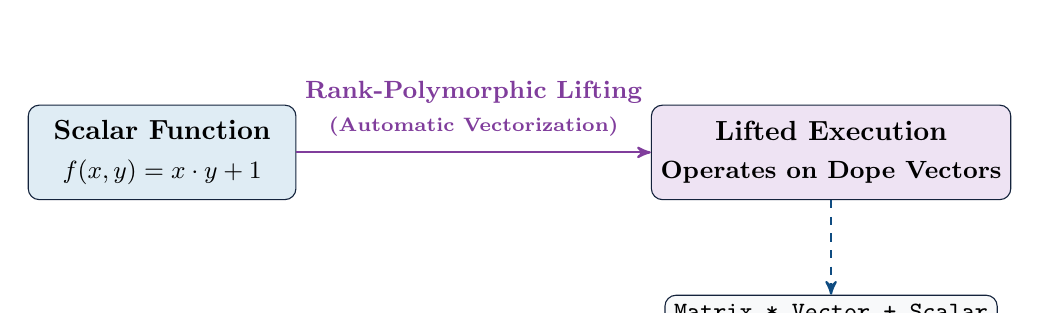
\begin{tikzpicture}[node distance=4.5cm, auto, >=stealth']
    \node [draw=sisalnavy, rounded corners=4pt, rectangle, fill=sisalblue!15, minimum width=3.4cm, minimum height=1.2cm, align=center, font=\bfseries] (scalar) {\textbf{Scalar Function}\\[2pt]\small $f(x, y) = x \cdot y + 1$};
    \node [draw=sisalnavy, rounded corners=4pt, rectangle, fill=sisalpurple!15, minimum width=3.6cm, minimum height=1.2cm, align=center, font=\bfseries, right=4.5cm of scalar] (matrix) {\textbf{Lifted Execution}\\[2pt]\small Operates on Dope Vectors};
    
    \draw [->, thick, sisalpurple!90!black] (scalar) -- node[above=2pt, font=\small\bfseries, align=center] {Rank-Polymorphic Lifting\\[1pt]\scriptsize (Automatic Vectorization)} (matrix);
    
    \node [draw=sisalnavy, rounded corners=4pt, fill=codebg, below=1.2cm of matrix, font=\small\ttfamily] (example) {Matrix * Vector + Scalar};
    \draw [->, dashed, thick, sisaldarkblue] (matrix) -- (example);
\end{tikzpicture}
\caption{Rank-Polymorphic Lifting in Sisal-2026.}
\label{fig:rank_poly_lifting}
\end{figure}

\section{Sisal-2026 Type Representation (\texttt{array\_dv[T]})}
In Sisal-2026, all dense multi-dimensional arrays use the single flat parameterized type \texttt{array\_dv[T]}.

\begin{note}[First Edition Specification: Exclusive \texttt{array\_dv} Support]
In the First Edition of the Sisal-2026 specification, the legacy \texttt{array} keyword is not supported. Only dense dope-vector arrays (\texttt{array\_dv}) are provided. Support for legacy ragged \texttt{array} representations may be evaluated for future editions of the language.
\end{note}

\begin{note}[Flat vs. Nested Type Syntax]
The dimensional rank (1D vector, 2D matrix, 3D tensor) of a dense rectangular array is a dynamic property stored in dope vector metadata at runtime, declared simply as \texttt{array\_dv[T]}. Nested type syntax like \texttt{array\_dv[array\_dv[T]]} is valid for constructing jagged arrays with non-uniform row lengths, but flat \texttt{array\_dv[T]} is the required representation for rank-polymorphic dense tensor computing.
\end{note}

Underneath, every \texttt{array\_dv[T]} value maps to the C++23 runtime structure:
\begin{lstlisting}[caption={\texttt{sisal\_array\_t} Dope Vector Structure}]
struct sisal_array_t {
    void* data;          // Pointer to contiguous element memory
    int32_t rank;        // Number of dimensions (1, 2, 3, ...)
    int32_t total_elems; // Total number of elements
    int32_t elem_size;   // Size of element T in bytes
    int32_t ref_count;   // Copy-on-Write reference counter
    int32_t* shape;      // Array of dimension sizes [dim_0, dim_1, ...]
    int32_t* stride;     // Array of byte strides [stride_0, stride_1, ...]
    int32_t offset;      // Element offset into contiguous buffer
};
\end{lstlisting}

\section{\texttt{array\_dv} Syntax, Benefits \& Potential Pitfalls: Flat vs. Nested Arrays}

While Sisal-2026 uses \texttt{array\_dv} as its primary array constructor, developers can instantiate arrays using two distinct structural models: \textbf{Flat Dope-Vector Arrays} (\texttt{array\_dv[T]}) and \textbf{Nested Jagged Arrays} (\texttt{array\_dv[array\_dv[T]]}). Understanding the syntax, runtime mechanics, benefits, and common pitfalls of each model is essential for writing high-performance dataflow code.

\subsection{1. Flat Dope-Vector Arrays (\texttt{array\_dv[T]})}
In Sisal-2026, the recommended representation for vectors, matrices, and high-rank tensors is a single flat parameterized type \texttt{array\_dv[T]}. The dimension rank (1D, 2D, 3D, etc.), shape sizes, and stride offsets are maintained at runtime inside the $O(1)$ \texttt{sisal\_array\_t} descriptor metadata.

\begin{itemize}
    \item \textbf{Declaration Syntax}: Declared simply as \texttt{type Matrix = array\_dv[double]}.
    \item \textbf{Indexing Syntax}: Indexed using multi-dimensional comma-separated subscripting: \texttt{A[i, j]} or \texttt{A[i, j, k]}.
    \item \textbf{Memory Representation}: Elements reside in a single, contiguous memory allocation. Accessing \texttt{A[i, j]} computes a linear offset $i \cdot \text{stride}_0 + j \cdot \text{stride}_1$ in $O(1)$ time without dereferencing inner row pointers.
    \item \textbf{Benefits}: Guarantees maximum cache locality, enables automatic SIMD vectorization and BLAS offloading, supports zero-copy slicing (\texttt{A[i, ..]}), and powers rank-polymorphic function lifting.
\end{itemize}

\subsection{2. Nested Jagged Arrays (\texttt{array\_dv[array\_dv[T]]})}
When a programmer writes a nested array type definition—such as \texttt{type IntArray = array\_dv[integer]} followed by \texttt{type JaggedGrid = array\_dv[IntArray]}—the Sisal-2026 compiler constructs an outer dope-vector array whose elements are themselves inner \texttt{sisal\_array\_t} descriptors (\texttt{sizeof(sisal\_array\_t)}).

Listing~\ref{lst:nested_array_demo} shows a complete working program utilizing nested \texttt{array\_dv} structures (\texttt{nested\_array\_dv.sis}).

\begin{lstlisting}[caption={Nested \texttt{array\_dv[array\_dv[T]]} Jagged Arrays (\texttt{nested\_array\_dv.sis})},label={lst:nested_array_demo}]
define Main

type IntArray = array_dv [integer]
type NestedArray = array_dv [IntArray]

function Main( returns integer, integer, integer )
  let
    % 1. Construct independent row vectors (varying lengths supported)
    Row1 := array [1: 10, 20, 30];  % 3 elements
    Row2 := array [1: 40, 50];      % 2 elements
    
    % 2. Construct outer dope-vector array storing inner array descriptors
    Grid := array [1: Row1, Row2];
    
    % 3. Access elements via intermediate row bindings
    R1 := Grid[1];
    R2 := Grid[2];
    Elem1 := R1[2]; % Returns Row1[2] = 20
    Elem2 := R2[1]; % Returns Row2[1] = 40
    Sz := array_size(Grid) % Returns 2 outer rows
  in
    Elem1, Elem2, Sz
  end let
end function
\end{lstlisting}

\subsection{3. Key Differences, Syntax Confusions \& Trade-Offs}

Table~\ref{tab:flat_vs_nested_array_dv} summarizes the structural differences between flat and nested dope-vector arrays in Sisal-2026.

\begin{table}[h!]
\centering
\small
\begin{tabularx}{\textwidth}{lXX}
\toprule
\textbf{Feature / Property} & \textbf{Flat \texttt{array\_dv[T]}} & \textbf{Nested \texttt{array\_dv[array\_dv[T]]}} \\
\midrule
\textbf{Type Declaration} & \texttt{type Matrix = array\_dv[double]} & \texttt{type Jagged = array\_dv[array\_dv[int]]} \\
\textbf{Buffer Layout} & Single contiguous memory block & Pointer array to separate inner descriptors \\
\textbf{Row Lengths} & Uniform rectangular ($M \times N$) & Non-uniform / Jagged supported \\
\textbf{Indexing Syntax} & Comma-separated: \texttt{Grid[i, j]} & Intermediate binding: \texttt{R := Grid[i]; R[j]} \\
\textbf{Chained Subscripting} & Not needed (\texttt{Grid[i, j]} used) & \texttt{Grid[1][2]} fails parsing; use \texttt{(Grid[1])[2]} \\
\textbf{Rank Polymorphism} & Supported automatically & Not supported (opaque nested descriptors) \\
\textbf{Cache \& Vectorization} & Optimal L1/L2 locality, SIMD/BLAS & Pointer indirection, no vectorization \\
\bottomrule
\end{tabularx}
\caption{Comparison of Flat vs. Nested \texttt{array\_dv} Representations.}
\label{tab:flat_vs_nested_array_dv}
\end{table}

\begin{tip}[Common Syntax Confusion: Chained Subscripting \texttt{Grid[1][2]}]
In standard Sisal grammar, writing \texttt{Grid[1][2]} directly on a single line produces a syntax parser error because \texttt{[2]} is not recognized as a trailing suffix on \texttt{Grid[1]}. To index into a nested jagged array, developers must use intermediate let-bindings (\texttt{R1 := Grid[1]; Elem := R1[2]}) or parenthesized subscripting \texttt{(Grid[1])[2]}.
\end{tip}

\begin{warning}[Performance Guidance: Prefer Flat \texttt{array\_dv[T]}]
While nested \texttt{array\_dv[array\_dv[T]]} structures compile and execute cleanly for irregular or jagged data collections, they introduce pointer indirection and forfeit rank polymorphism, zero-copy slicing, and SIMD vectorization. Developers should use flat \texttt{array\_dv[T]} for all dense linear algebra and tensor computations, reserving nested arrays strictly for non-uniform data structures.
\end{warning}

\section{Sisal-2026 Rank-Polymorphic Examples}

\subsection{1. Matrix-Vector \& Matrix-Scalar Operations}
In Sisal-2026, rank polymorphism operates on \texttt{array\_dv[T]} arguments along with scalar values. Built-in binary operators (\texttt{+}, \texttt{-}, \texttt{*}, \texttt{/}) and functions accepting \texttt{array\_dv} arguments inspect the dynamic rank metadata of their inputs and lift automatically across higher-dimensional dope vectors:

\begin{lstlisting}[caption={Rank-Polymorphic Matrix-Vector \& Scalar Expressions}]
function TransformAndScale( M : array_dv[real]; V : array_dv[real]; s : real returns array_dv[real] )
  let
    % M is a 2D Matrix of Shape [2, 3]
    % V is a 1D Vector of Shape [3]
    % s is a scalar real (0D)
    
    % 1. Matrix + Vector broadcast addition -> returns Shape [2, 3]
    M_plus_V := M + V;
    
    % 2. Matrix-Scalar broadcast multiplication -> returns Shape [2, 3]
    Scaled := M_plus_V * s;
    
    % 3. Combined inline rank-polymorphic expression
    Result := (M * s) + V
  in
    Result
  end let
end function
\end{lstlisting}

\begin{note}[Rank-Polymorphic Operand Scope]
Rank-polymorphic lifting applies directly to built-in operators and functions defined with \texttt{array\_dv[T]} parameters (along with scalar values). To apply a scalar-only function \texttt{f(x, y : real)} over array elements, use the whole-array \texttt{MAP(A, B, f)} primitive or define the function signature with \texttt{array\_dv[real]} parameters.
\end{note}

\section{Array Construction: Flat 1D Literals \& \texttt{reshape}}
Array literal syntax \texttt{array\_dv [1: v1, v2, ...]} constructs a \textbf{1D flat vector}. To construct a multi-dimensional matrix or tensor from literal values in Sisal-2026, developers initialize a flat 1D vector literal and reshape it using the built-in \texttt{reshape(A, dim0, dim1, ...)} function, or construct it dynamically via parallel \texttt{forall} loop gather reductions.

\begin{lstlisting}[caption={Multi-Dimensional Array Construction via \texttt{reshape}}]
function MatrixInit( returns array_dv[real] )
  let
    % 1. Construct a flat 1D vector literal (16 elements)
    Flat := array_dv [1: 1.0, 2.0, 3.0, 4.0, 
                         5.0, 6.0, 7.0, 8.0, 
                         9.0, 10.0, 11.0, 12.0, 
                         13.0, 14.0, 15.0, 16.0];
                         
    % 2. Reshape into a 4x4 rank-2 matrix (O(1) dope vector view shift)
    M := reshape(Flat, 4, 4)
  in
    M
  end let
end function
\end{lstlisting}

\subsection{2. Zero-Copy Slicing \& Explicit Range Notation}
Slicing a matrix creates a zero-copy metadata view with $O(1)$ constant time complexity:

\begin{lstlisting}[caption={Zero-Copy Slicing in Sisal-2026}]
function SlicingDemo( returns array_dv[real] )
  let
    % Construct 4x4 Matrix by reshaping flat 1D literal
    Flat := array_dv [1: 1.0, 2.0, 3.0, 4.0, 5.0, 6.0, 7.0, 8.0, 
                         9.0, 10.0, 11.0, 12.0, 13.0, 14.0, 15.0, 16.0];
    M := reshape(Flat, 4, 4);
                      
    % Sub-matrix view (Rows 2..3, Cols 1..2) -> Shape [2, 2]
    SubView := M[2..3, 1..2];
    
    % Explicit row slice using range notation: Extract row 2 -> 1D Vector of Shape [4]
    RowVector := M[2, 1..4]
  in
    SubView + RowVector % Automatic broadcasting!
  end let
end function
\end{lstlisting}

\section{Indexing Ambiguity \& Explicit Slicing Notation (\texttt{A[i]} vs. \texttt{A[i, ..]})}
A fundamental design decision in Sisal-2026 is disambiguating single-subscript indexing vs. slicing.

\subsection{The Lowering Problem with \texttt{A[i]}}
In legacy ragged array languages (such as Sisal 1.2 or C nested arrays), a 2D matrix is an array of pointers (\texttt{array[array[T]]}). In that pointer model, single-index access \texttt{A[i]} dereferences the outer pointer to return a 1D row array \texttt{array[T]}.

However, in Sisal-2026, all dense arrays use flat dope vectors (\texttt{array\_dv[T]}). If single-subscript indexing \texttt{A[i]} were allowed to return a 1D row vector when \texttt{A} is a 2D matrix, but a scalar \texttt{T} when \texttt{A} is a 1D vector, the IF1 IR lowering and static type checking of \texttt{A[i]} would be ambiguous:
\begin{itemize}
    \item Does \texttt{A[i]} lower to a scalar element access (\texttt{DOPE\_VECTOR\_ELEMENT}) or a multi-element slice view (\texttt{DOPE\_VECTOR\_SLICE})?
    \item What is the static return type of \texttt{A[i]} in the compiler type checker?
\end{itemize}

\subsection{The Sisal-2026 Solution}
Sisal-2026 enforces strict, deterministic syntax rules:
\begin{enumerate}
    \item \textbf{Single Subscript Indexing (\texttt{A[i]})}: \textbf{ALWAYS returns a scalar value \texttt{T}}!
    \begin{itemize}
        \item For a 1D vector \texttt{V}, \texttt{V[i]} returns the $i$-th scalar element.
        \item For a 2D matrix \texttt{M}, single-subscript \texttt{M[i]} performs \textbf{linear (flat 1D) indexing} into the underlying row-major memory buffer as if \texttt{M} were a single flattened 1D row! Thus, \texttt{M[i]} extracts the $i$-th scalar element of the flat matrix.
        \item 2D coordinate scalar access uses two-subscript indexing \texttt{M[i, j]}.
    \end{itemize}
    \item \textbf{Explicit Row/Column Slicing (\texttt{A[i, ..]} or \texttt{A[i, 1..N]})}: To explicitly extract a 1D row vector slice from a 2D matrix, developers use range slicing notation \textbf{\texttt{A[i, ..]}} or \textbf{\texttt{A[i, 1..N]}}.
\end{enumerate}

\begin{lstlisting}[caption={Indexing vs. Explicit Slicing in Sisal-2026}]
function IndexVsSliceDemo( M : array_dv[real] returns real, array_dv[real] )
  let
    % 1. Coordinate Indexing: M[2, 3] ALWAYS returns a scalar real element
    scalar_val := M[2, 3];
    
    % 2. Explicit Row Slicing: M[2, ..] explicitly extracts Row 2 as a 1D Vector view
    row_slice := M[2, ..];
    
    % 3. Explicit Column Slicing: M[.., 3] explicitly extracts Column 3 as a 1D Vector view
    col_slice := M[.., 3]
  in
    scalar_val, row_slice
  end let
end function
\end{lstlisting}

\begin{tip}[Why This Is a Major Architectural Advantage]
Enforcing that \texttt{M[i, j]} is scalar element access while \texttt{M[i, ..]} is slice view extraction eliminates type ambiguity in the compiler frontend. The type checker statically knows whether an expression produces a scalar \texttt{T} or a metadata dope vector view \texttt{array\_dv[T]}, leading to clean IF1 node lowering and zero runtime type-check overhead.
\end{tip}

\section{Broadcasting Rules: Right-Aligned Trailing Axis Agreement}
Sisal-2026 enforces right-aligned trailing axis broadcasting rules (matching NumPy and PyTorch conventions):

\begin{figure}[h!]
\centering
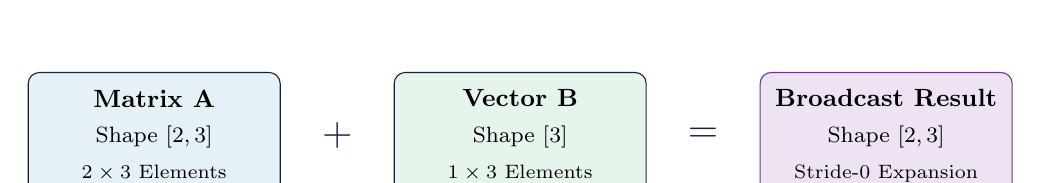
\begin{tikzpicture}[
    box/.style={draw=sisalnavy, rounded corners=4pt, minimum height=1.6cm, minimum width=3.2cm, align=center, font=\small},
    op/.style={font=\Large\bfseries\color{sisalnavy}}
]
    % Matrix A Card
    \node[box, fill=sisalblue!12] (matA) {
        \textbf{Matrix A}\\[2pt]
        \footnotesize Shape $[2, 3]$\\[2pt]
        \scriptsize $2 \times 3$ Elements
    };

    % Plus Operator
    \node[op, right=0.4cm of matA] (plus) {$+$};

    % Vector B Card
    \node[box, fill=sisalgreen!12, right=0.4cm of plus] (vecB) {
        \textbf{Vector B}\\[2pt]
        \footnotesize Shape $[3]$\\[2pt]
        \scriptsize $1 \times 3$ Elements
    };

    % Equals Operator
    \node[op, right=0.4cm of vecB] (equals) {$=$};

    % Result Broadcast Card
    \node[box, fill=sisalpurple!15, draw=sisalpurple!80!black, right=0.4cm of equals] (result) {
        \textbf{Broadcast Result}\\[2pt]
        \footnotesize Shape $[2, 3]$\\[2pt]
        \scriptsize Stride-0 Expansion
    };
\end{tikzpicture}
\caption{Right-Aligned Stride-0 Broadcasting Alignment.}
\label{fig:broadcasting_alignment}
\end{figure}

When evaluating $A \oplus B$:
\begin{enumerate}
    \item \textbf{Right Alignment}: Align dimension shapes starting from the rightmost (trailing) axis.
    \item \textbf{Axis Compatibility}: For each aligned axis $d$:
    \begin{itemize}
        \item If \texttt{shape\_A[d] == shape\_B[d]}, the dimensions agree.
        \item If one dimension size is $1$, it is expanded to match the other size by setting its byte stride to $0$.
        \item If dimension sizes differ and neither is $1$, a runtime shape error is raised.
    \end{itemize}
    \item \textbf{Zero-Copy Stride-0 Expansion}: Axis expansion incurs $0$ byte copies because setting \texttt{stride = 0} reuses existing element memory repeatedly without duplication.
\end{enumerate}

\section{IF1 Compiler Lowering \& Execution Pass}
During AST lowering to the IF1 dataflow graph:
\begin{enumerate}
    \item Binary arithmetic operations between \texttt{array\_dv} operands lower to \texttt{CONFORM\_CHECK} nodes.
    \item \texttt{CONFORM\_CHECK} verifies shape compatibility and calculates output shape and stride-0 metadata.
    \item Elementwise computation loops iterate over total elements using \texttt{sisal\_dv\_offset\_at} to compute flat memory addresses.
\end{enumerate}

\begin{lstlisting}[caption={C++23 Runtime Stride-0 Index Calculation}]
inline int32_t sisal_dv_offset_at(const sisal_array_t* arr, int32_t flat_idx) {
    int32_t offset = arr->offset;
    int32_t rem = flat_idx;
    for (int32_t i = 0; i < arr->rank; ++i) {
        int32_t dim_size = arr->shape[i];
        int32_t coord = rem / arr->stride_mod[i];
        rem %= arr->stride_mod[i];
        % Stride of 0 automatically zeroes out offset addition for broadcast axes!
        offset += coord * arr->stride[i];
    }
    return offset;
}
\end{lstlisting}

\section{Summary of Benefits in Sisal-2026}
\begin{table}[h!]
\centering
\begin{tabularx}{\textwidth}{lXX}
\toprule
\textbf{Feature} & \textbf{Legacy Sisal 1.2 / 2.0} & \textbf{Sisal-2026 (\texttt{array\_dv})} \\
\midrule
Memory Layout & Ragged nested pointers (\texttt{array[array[T]]}) & Contiguous flat buffer with $O(1)$ dope vector \\
Slicing Cost & $O(N)$ allocation \& copying & $O(1)$ constant-time metadata view shift \\
Broadcasting & Manual nested \texttt{forall} loops & Automatic right-aligned zero-copy stride-0 \\
Single Assignment & Static update-in-place pass & Native Copy-on-Write reference counting \\
Hardware Acceleration & Manual vectorization & Direct BLAS/LAPACK (\texttt{cblas\_dgemm}) \\
\bottomrule
\end{tabularx}
\caption{Comparison of Array Models.}
\label{tab:array_comparison}
\end{table}

\chapter{Expressions, Operators \& SIMD Intrinsics}
\label{chap:expressions_operators}

\section{Arithmetic, Relational \& Logical Expressions}
Sisal-2026 supports standard mathematical operators with traditional precedence rules:

\begin{table}[h!]
\centering
\begin{tabularx}{\textwidth}{llX}
\toprule
\textbf{Category} & \textbf{Operators} & \textbf{Description} \\
\midrule
Arithmetic & \texttt{+}, \texttt{-}, \texttt{*}, \texttt{/}, \texttt{**}, \texttt{mod} & Addition, Subtraction, Multiplication, Division, Power, Modulo \\
Relational & \texttt{=}, \texttt{\textasciitilde=}, \texttt{<}, \texttt{<=}, \texttt{>}, \texttt{>=} & Equal, Not Equal, Less, Less-Equal, Greater, Greater-Equal \\
Logical & \texttt{and}, \texttt{or}, \texttt{not} & Boolean operations \\
Bitwise & \texttt{bit\_and}, \texttt{bit\_or}, \texttt{bit\_xor} & Low-level bitwise operations \\
\bottomrule
\end{tabularx}
\caption{Operator Precedence \& Categories.}
\label{tab:operators}
\end{table}

\section{Pattern Matching \& Wildcard Bindings}
\label{sec:wildcard}
Sisal-2026 introduces pattern matching with wildcard (\texttt{\_}) support in \texttt{let} bindings, assignment expressions, and function returns:

\begin{lstlisting}[caption={Wildcard Pattern Matching Examples}]
function TupleUnpack( returns integer, real, boolean )
  10, 3.14, true
end function

function Main( returns integer )
  let
    % Ignore second return value using wildcard _
    val, _, flag := TupleUnpack();
    _ := printf("Flag value: %d\n", if flag then 1 else 0 end if)
  in
    val
  end let
end function
\end{lstlisting}

\section{First-Class Higher-Order Functions (HOFs) \& Closures}
Functions in Sisal-2026 are first-class values. Lambda expressions create functional closures that capture environment variables:

\begin{lstlisting}[caption={Higher-Order Function \& Closure Usage}]
function ApplyTwice( f : function(integer returns integer); x : integer returns integer )
  f(f(x))
end function

function TestHOF( returns integer )
  let
    multiplier := 5;
    % Lambda closure capturing multiplier
    scale := function( v : integer returns integer ) v * multiplier end function;
    res := ApplyTwice(scale, 2) % Computes (2 * 5) * 5 = 50
  in
    res
  end let
end function
\end{lstlisting}

\section{Hardware SIMD Intrinsics (\texttt{float4}, \texttt{mat2})}
To exploit CPU vector execution units (ARM Neon, x86 AVX-512) and GPU shader cores, Sisal-2026 introduces fixed-size SIMD vector and matrix types:

\begin{table}[h!]
\centering
\begin{tabular}{lll}
\toprule
\textbf{SIMD Type} & \textbf{Components} & \textbf{Target Alignment} \\
\midrule
\texttt{float2}, \texttt{int2} & 2 single-precision floats / ints & 64-bit SIMD lane \\
\texttt{float3} & 3 single-precision floats & 96-bit SIMD lane \\
\texttt{float4}, \texttt{int4} & 4 single-precision floats / ints & 128-bit SIMD lane \\
\texttt{mat2} & $2 \times 2$ matrix & 128-bit SIMD matrix register \\
\texttt{mat3} & $3 \times 3$ matrix & 288-bit SIMD register block \\
\texttt{mat4} & $4 \times 4$ matrix & 512-bit SIMD register block \\
\bottomrule
\end{tabular}
\caption{Fixed SIMD Vector \& Matrix Primitives.}
\label{tab:simd_types}
\end{table}

\begin{lstlisting}[caption={SIMD Math Intrinsics Example}]
function TransformVector( v : float4; m : mat4 returns float4 )
  let
    % Direct SIMD matrix-vector multiplication compiled to single AVX/Neon instruction
    v_out := m * v;
    norm  := dot(v_out, v_out)
  in
    v_out
  end let
end function
\end{lstlisting}

\chapter{Einstein Summation \& Bulk Array Operations}
\label{chap:einsum_bulk_ops}

\section{Einstein Summation Engine (\texttt{EINSUM})}
Sisal-2026 includes a built-in Einstein summation contraction engine. The syntax parses standard multi-tensor subscript notation:

\begin{lstlisting}[caption={Einstein Summation Syntax}]
C := EINSUM("ij,jk->ik", MatrixA, MatrixB)
\end{lstlisting}

\subsection{Lowering Fast-Paths}
The compiler inspects \texttt{EINSUM} subscript strings during AST lowering (\texttt{einsum\_lower.ml}) and routes contractions to hardware BLAS fast-paths:
\begin{itemize}
    \item \texttt{"ij,jk->ik"}: Matrix-Matrix Multiplication $\rightarrow$ \texttt{cblas\_dgemm} / \texttt{cblas\_sgemm}.
    \item \texttt{"ij,j->i"}: Matrix-Vector Multiplication $\rightarrow$ \texttt{cblas\_dgemv} / \texttt{cblas\_sgemv}.
    \item \texttt{"i,i->"}: Vector Dot Product $\rightarrow$ \texttt{cblas\_ddot} / \texttt{cblas\_sdot}.
    \item \texttt{"ij->ji"}: Matrix Transposition $\rightarrow$ $O(1)$ stride swap in dope vector metadata.
\end{itemize}

For general multi-index contractions not matching single 2D BLAS signatures, the compiler lowers the expression to an IF1 \texttt{EINSUM\_NODE} multi-loop iteration graph.

\subsection{High-Rank Tensors \& Contraction Path Optimization}
While \texttt{MATMUL} and \texttt{INNERPRODUCT} provide direct, concise syntax for standard 2D matrix operations, \texttt{EINSUM} serves two critical structural roles in tensor compilation:
\begin{enumerate}
    \item \textbf{High-Rank Tensor Contractions}: For 3D, 4D, and 5D attention graphs (e.g. $Q, K, V \in \mathbb{R}^{B \times H \times S \times D}$ in Grouped Query Attention), \texttt{EINSUM("bhqd,bhkd->bhqk", Q, K)} declaratively specifies contraction axes without manual reshape or permutation boilerplate.
    \item \textbf{Multi-Contraction Chain Optimization (Compiler Roadmap Target)}: When chaining multiple matrix/tensor products in sequence (e.g., $P \cdot V \cdot W_O$), exposing the contraction topology through \texttt{EINSUM} provides the structural foundation for \textbf{Dynamic Programming Contraction Path Optimization} (on the compiler optimizer roadmap). This pass will automatically evaluate intermediate tensor dimension products to select the optimal parenthesization order that minimizes total FLOP complexity (reducing $O(N^4)$ naive contractions down to optimal $O(N^3)$ sequences) before emitting BLAS kernel calls.
\end{enumerate}

\subsection{Tiled EINSUM Subscripts \& Unified Permutation (Wishlist Item)}
An upcoming design proposal on the Sisal-2026 compiler wishlist extends the \texttt{EINSUM} subscript string to natively unify \textbf{tensor contraction math}, \textbf{L1/L2 cache tiling}, and \textbf{loop permutation} into a single bracketed notation, eliminating separate imperative transformation scripts.

In this syntax, bracket nesting depth represents tile/cache depth (e.g. \texttt{(i 32)} represents a 32-element L2 block tile), while the left-to-right order of terms on the output side (\texttt{->}) dictates the execution loop nesting:

\begin{lstlisting}[language=Sisal,caption={Tiled EINSUM Subscript with Middle $k$ Loop}]
% Tiled Matrix Multiplication (32x64x16) with k as Middle Loop
C := EINSUM("((i 32) (j 64)) ((j 64) (k 16)) -> (i 32) (k 16) (j 64)", A, B)
\end{lstlisting}

\subsubsection{Step-by-Step Lowering Walkthrough (Pseudo-Fortran)}

To understand why placing $k$ as the middle loop delivers superior performance, consider the step-by-step compiler lowerings from naive untiled execution down to tiled $k$-in-the-middle micro-kernels:

\begin{enumerate}
    \item \textbf{Naive Untiled Lowering (\texttt{"ik, kj -> ij"} $\rightarrow$ $i \rightarrow j \rightarrow k$ order)}:
\begin{lstlisting}[language=Fortran]
! Naive Lowering: Reduction k in innermost loop (Strided access on B)
DO i = 1, M
   DO j = 1, N
      sum_val = 0.0d0
      DO k = 1, K
         sum_val = sum_val + A(i, k) * B(k, j)   ! B(k, j) jumps N elements every step
      END DO
      C(i, j) = sum_val
   END DO
END DO
\end{lstlisting}

    \item \textbf{Interchanged Lowering ($k$ as Middle Loop $\rightarrow$ $i \rightarrow k \rightarrow j$ order)}:
\begin{lstlisting}[language=Fortran]
! Interchanged: k in middle position (Scalar broadcast of A, unit-stride for B and C)
DO i = 1, M
   DO k = 1, K                       ! k is MIDDLE loop!
      a_val = A(i, k)                ! Broadcast: Load once into register
      DO j = 1, N                    ! Innermost loop over j (Vector unit-stride)
         C(i, j) = C(i, j) + a_val * B(k, j)
      END DO
   END DO
END DO
\end{lstlisting}

    \item \textbf{Tiled Lowering with $k$ in Middle (\texttt{"((i 32) (j 64)) ((j 64) (k 16)) -> (i 32) (k 16) (j 64)"})}:
\begin{lstlisting}[language=Fortran]
! Tiled & Interchanged: i_tile -> k_tile -> j_tile -> i_elem -> k_elem -> j_elem
DO i_tile = 1, M, 32
   DO k_tile = 1, K, 16                 ! k_tile is MIDDLE tile loop!
      DO j_tile = 1, N, 64
         
         ! Inner Micro-kernel (L1 Cache / SIMD Vector Registers)
         DO i_elem = i_tile, MIN(i_tile + 31, M)
            DO k_elem = k_tile, MIN(k_tile + 15, K)   ! k_elem is MIDDLE element loop!
               a_val = A(i_elem, k_elem)
               
               !DIR$ SIMD (Vectorized unit-stride loop over j_elem)
               DO j_elem = j_tile, MIN(j_tile + 63, N)
                  C(i_elem, j_elem) = C(i_elem, j_elem) + a_val * B(k_elem, j_elem)
               END DO
            END DO
         END DO

      END DO
   END DO
END DO
\end{lstlisting}

    \item \textbf{3D Batched MatMul \& 4D Attention Lowering (\texttt{"b ((m 32) (k 16)) (b ((k 16) (n 64))) -> b (m 32) (k 16) (n 64)"})}:
\begin{lstlisting}[language=Fortran]
! 3D Batched MatMul with Parallel Batch (b) & Middle k Loop
!$OMP PARALLEL DO COLLAPSE(2) PRIVATE(m_elem, k_elem, n_elem, a_val)
DO b = 1, B
   DO m_tile = 1, M, 32
      DO k_tile = 1, K, 16                 ! k_tile is MIDDLE tile loop!
         DO n_tile = 1, N, 64
            
            ! Inner Micro-kernel (Fits 100% in L1 Cache)
            DO m_elem = m_tile, MIN(m_tile + 31, M)
               DO k_elem = k_tile, MIN(k_tile + 15, K)   ! k_elem is MIDDLE element loop!
                  a_val = A(b, m_elem, k_elem)
                  
                  !DIR$ SIMD
                  DO n_elem = n_tile, MIN(n_tile + 63, N)
                     C(b, m_elem, n_elem) = C(b, m_elem, n_elem) + a_val * B(b, k_elem, n_elem)
                  END DO
               END DO
            END DO

         END DO
      END DO
   END DO
END DO
!$OMP END PARALLEL DO
\end{lstlisting}
    For 4D Transformer Attention ($Q \cdot K^T$ with Batch $b$, Heads $h$, Sequence $s$, Head Dim $d$), writing \texttt{Scores := EINSUM("b h ((s 64) (d 16)) (b h ((k 64) (d 16))) -> b h (s 64) (d 16) (k 64)", Q, K)} lowers to thread-parallel batch execution over $(b, h)$, outer tiles over Query sequence $(s)$, \textbf{head dimension $d$ reduced in middle registers}, and Key sequence $(k)$ streamed with unit-stride vector memory access.
\end{enumerate}

\subsubsection{Related Work \& Novelty Analysis}

A comparison of the Sisal-2026 tiled \texttt{EINSUM} proposal with state-of-the-art tensor compilers and programming frameworks highlights its unique design positioning:

\begin{itemize}
    \item \textbf{NumPy / PyTorch \texttt{einsum}}: Uses standard Einstein notation (\texttt{"ik,kj->ij"}). Expresses contraction math declaratively, but has \textbf{zero syntax for loop tiling, cache block sizes, or execution loop ordering}.
    \item \textbf{Halide (Ragan-Kelley et al., PLDI 2013) \& TVM (Chen et al., OSDI 2018)}: Pioneered the decoupling of computation algorithms from execution schedules. However, scheduling is imperative and separate from the math expression (e.g. \texttt{s.tile(i, i\_out, i\_in, 32).reorder(i\_out, k\_out, j\_out)} in an external Python script).
    \item \textbf{Einops (Rozenberg, ICLR 2022)}: Provides index rearrangement syntax (\texttt{"b (h w) -> b h w"}), but focuses exclusively on spatial array reshaping and tensor broadcasting---\textbf{cannot specify contraction reductions, cache block sizes, or SIMD loop order}.
    \item \textbf{Tensor Comprehensions (Vasilache et al., FAIR 2018) \& TACO (Kjolstad et al., OOPSLA 2017)}: Uses polyhedral compiler infrastructure (ISL) to discover tile sizes automatically during compilation. No inline syntax exists for the developer to specify tile bounds directly in the string.
    \item \textbf{Sisal-2026 Novelty}:
    \begin{enumerate}
        \item \textbf{Purely Functional Inline Scheduling}: Unifies math definition and hardware loop schedule in a single functional string expression.
        \item \textbf{Zero-Keyword Positional Ordering}: The position of bracketed terms on the RHS of \texttt{->} dictates outer/inner loop nesting and loop interchange (e.g. \texttt{-> (i 32) (k 16) (j 64)} places $k$ in the middle).
        \item \textbf{Cache Depth Mapping}: Bracket depth corresponds 1-to-1 to physical memory levels: \texttt{i} (flat DRAM), \texttt{(i 32)} (L2 Cache), \texttt{((i 128) 8)} (L1 / Vector Register).
    \end{enumerate}
\end{itemize}

\subsection{Higher-Order Epilogue \& Pre-Processing Fusion in EINSUM (Wishlist Item)}
Activation functions and transformations (such as \texttt{SwiGLU}, \texttt{Swish}, \texttt{GELU}, \texttt{ReLU}, \texttt{SiLU}, \texttt{RMSNorm}, \texttt{RoPE}, \texttt{BiasAdd}) can be captured \textbf{directly inside the subscript string} as named tokens without needing to pass them as extra function arguments to \texttt{EINSUM}:

\begin{lstlisting}[language=Sisal,caption={Fused SwiGLU FFN via EINSUM in Sisal-2026}]
function FusedSwiGLUFFN( X, W1, W2, W3 : array_dv[double] returns array_dv[double] )
  let
    % Activation token SwiGLU captured inside the string -- ZERO extra function args!
    Hidden := EINSUM(
      "((s 32) (h 64)) ((h 64) (d 16)), ((s 32) (h 64)) ((h 64) (d 16)) -> (s 32) (d 16) ((h 64) SwiGLU)",
      X, W1, X, W2
    )
  in
    EINSUM("((s 32) (d 16)) ((d 16) (h 64)) -> (s 32) (h 64) (d 16)", Hidden, W3)
  end let
end function
\end{lstlisting}

The subscript parser (\texttt{einsum\_lower.ml}) resolves built-in activation tokens or in-scope function identifiers directly from the AST symbol table. This unifies (1) tensor contraction math, (2) L1/L2 cache tiling, (3) loop interchange, (4) pre-processing load transformations, and (5) post-processing store activations \textbf{all inside a single self-contained \texttt{EINSUM} expression}!

\begin{note}[Work-in-Progress Disclaimer]
This documentation and manual are works in progress. Because compiler optimization passes, AST lowerings, and backend code generators are actively evolving, developers should examine the execution logs, generated C++ files, and benchmark results in \texttt{test/e2e/} to inspect the authoritative current state of the compiler's optimization capabilities.
\end{note}


\section{APL-Style Bulk Operations Battery (58 Primitives)}
Sisal-2026 provides 58 whole-array bulk primitives, eliminating manual parallel \texttt{forall} boilerplate code for standard array manipulations:

\begin{table}[h!]
\centering
\small
\begin{tabularx}{\textwidth}{l >{\raggedright\arraybackslash}p{4.0cm} >{\raggedright\arraybackslash}X}
\toprule
\textbf{Category} & \textbf{Primitive Names} & \textbf{Semantics \& Description} \\
\midrule
Reductions & \texttt{SUM}, \texttt{PRODUCT}, \texttt{LEAST}, \texttt{GREATEST}, \texttt{MEAN}, \texttt{VARIANCE}, \texttt{STDDEV}, \texttt{NORM} & Reduce array along default or specified axis into scalar value. \\
\addlinespace
Scans & \texttt{SCAN}, \texttt{CUMSUM}, \texttt{CUMPROD} & Prefix scan operation along leading axis. \\
\addlinespace
Structural & \texttt{TAKE}, \texttt{DROP}, \texttt{ROTATE}, \texttt{REVERSE}, \texttt{COMPRESS}, \texttt{RAVEL}, \texttt{EXPAND}, \texttt{SQUEEZE}, \texttt{PERMUTE} & Structural reshaping and axis permuting operations. \\
\addlinespace
Selection & \texttt{SORT}, \texttt{ARGMAX}, \texttt{ARGMIN}, \texttt{GRADE\_UP}, \texttt{GRADE\_DOWN}, \texttt{NONZERO}, \texttt{WHERE} & Sorting and index mask extraction. \\
\addlinespace
Higher-Order & \texttt{MAP}, \texttt{FOLDL}, \texttt{FOLDR}, \texttt{STENCIL}, \texttt{INNERPRODUCT}, \texttt{OUTERPRODUCT} & Functional combinators across multidimensional dope vectors. \\
\bottomrule
\end{tabularx}
\caption{APL Bulk Operation Battery Summary.}
\label{tab:bulk_ops}
\end{table}

\begin{lstlisting}[caption={Bulk Operation Battery Code Examples}]
let
  A := array_dv [1: 5.0, 2.0, 9.0, 1.0, 7.0];
  
  % Calculate Mean and Standard Deviation
  m := MEAN(A);
  s := STDDEV(A);
  
  % Sort and Grade Indices
  SortedA := SORT(A);          % [1.0, 2.0, 5.0, 7.0, 9.0]
  MaxIdx  := ARGMAX(A);        % 3 (index of value 9.0)
  
  % Stencil Convolution
  Smooth := STENCIL(A, 3, function(window : array_dv[real] returns real)
    (window[1] + window[2] + window[3]) / 3.0
  end function)
in
  SortedA, MaxIdx, Smooth
end let
\end{lstlisting}

\chapter{Parallel \& Sequential Loops}
\label{chap:loops_forall}

\section{Parallel Loops (\texttt{for})}
The parallel \texttt{for} loop (lowered to \texttt{ForallNode} compound graphs in IF1 IR) is the primary construct for data-parallel execution in Sisal-2026. Every iteration of a parallel \texttt{for} loop is independent and can execute concurrently on separate CPU worker threads or GPU thread blocks.

\begin{note}[Keyword Clarification: \texttt{for} vs. \texttt{forall}]
In Sisal-2026 source code, the keyword for parallel loops is \textbf{\texttt{for}} (e.g., \texttt{for i in 1..N ... end for}). The term \emph{forall} refers to the underlying IF1 dataflow compound graph node (\texttt{ForallNode}) and literature terminology.
\end{note}

\subsection{Syntax \& Generator Ranges}
A parallel \texttt{for} loop consists of three sections:
\begin{enumerate}
    \item \textbf{Generator Range}: Defines the index domain (\texttt{i in 1, N} or element iteration \texttt{x in Array}).
    \item \textbf{Loop Body}: Computes expression bindings for each element in the domain.
    \item \textbf{Returns Clause}: Specifies reduction accumulators (\texttt{sum of}, \texttt{array of}, \texttt{stream of}, \texttt{product of}, \texttt{least of}, \texttt{greatest of}).
\end{enumerate}

\begin{lstlisting}[caption={Parallel \texttt{for} Loop Example}]
function VectorScale( A : array_dv[real]; factor : real returns array_dv[real] )
  for x in A
    y := x * factor
  returns
    array of y
  end for
end function
\end{lstlisting}

\subsection{Cross Products \& Dot Products}
Multiple generator ranges can be combined using \texttt{cross} (Cartesian product) or \texttt{dot} (lock-step parallel iteration):

\begin{lstlisting}[caption={Cross Product vs. Dot Product Generators}]
% Cross Product (N x M iterations)
Matrix := for i in 1, N cross j in 1, M
  val := i * 10 + j
returns
  array of val
end for;

% Dot Product (min(N, M) lock-step iterations)
Sums := for x in VectorA dot y in VectorB
  z := x + y
returns
  array of z
end for;
\end{lstlisting}

\section{Sequential Loops (\texttt{for initial})}
When loop iterations have loop-carried dependencies (where iteration $k$ requires results from iteration $k-1$), the \texttt{for initial} sequential loop is used.

\begin{lstlisting}[caption={Sequential Loop with Zero-Copy Tuple Swapping}]
function Fibonacci( n : integer returns integer )
  for initial
    i := 1;
    a := 0;
    b := 1
  while i < n repeat
    i := old i + 1;
    a := old b;
    b := old a + old b
  returns
    value of b
  end for
end function
\end{lstlisting}

\begin{note}[\texttt{old} Keyword]
Inside a \texttt{for initial} loop body, the \texttt{old} keyword references value bindings from the previous iteration. The compiler lowers state updates to zero-copy pointer swaps.
\end{note}

\section{Loop Semantics \& Comparative Analysis: Sisal vs. C vs. Fortran}
Sisal's \texttt{for initial} construct is a functional state-transition graph loop rather than a control-flow jump. This fundamental semantic difference distinguishes Sisal loops from traditional imperative loops in C and Fortran.

\subsection{Core Rules of \texttt{for initial} Iteration}
\begin{enumerate}
    \item \textbf{Rule 1: Unconditional Initial Seed Evaluation (No Undefined States)}:
    Sisal defines a single-assignment value history that begins with an explicit initial state (\texttt{body\_0}). The \texttt{initial} seed is unconditionally evaluated and added to any accumulation collection (e.g. \texttt{returns stream of I}) \emph{before} the loop condition check occurs. Even in a zero-trip loop where the condition is false on entry, the initial seed value is safely defined and gathered, eliminating any risk of reading garbage or uninitialized memory.
    
    \item \textbf{Rule 2: Out-of-Bounds Value Calculation \& Gathering}:
    In Sisal, the loop body computes the new state of loop variables from the previous state (\texttt{I := old I + step}). If the condition is satisfied, the body computes the new state and immediately gathers it. Consequently, the final value of \texttt{I} (which fails the subsequent condition check and terminates the loop) has already been computed and gathered into the result collection.
\end{enumerate}

\subsection{Comparative Analysis: Zero-Trip \& Normal Loops}
Table~\ref{tab:loop_comparison_zero_trip} and Table~\ref{tab:loop_comparison_normal} compare the execution behavior of Sisal, C/C++, and Fortran under zero-trip and normal loop scenarios.

\begin{table}[h!]
\centering
\small
\begin{tabularx}{\textwidth}{l >{\raggedright\arraybackslash}p{4.2cm} >{\raggedright\arraybackslash}X}
\toprule
\textbf{Language} & \textbf{Example Syntax} & \textbf{Execution Details \& Undefined Risk} \\
\midrule
\textbf{Sisal-2026} & \texttt{for initial I := 10 while I < 5 repeat I := old I + 1 returns stream of I end for} & Initial seed executes unconditionally and gathers \texttt{10}. Condition \texttt{10 < 5} is false $\rightarrow$ exits. \\
\addlinespace
& & \textbf{Stream}: \texttt{[10]} (Size 1) \quad \textbf{Risk}: None. \\
\midrule
\textbf{C / C++} & \texttt{int r; for(int i=10; i<5; i++) r=i;} & Condition \texttt{10 < 5} is checked first and fails. Body never executes. \\
\addlinespace
& & \textbf{Vector}: \texttt{[]} (Empty) \quad \textbf{Risk}: High (reading \texttt{r} yields garbage/UB). \\
\midrule
\textbf{Fortran} & \texttt{INTEGER :: I, R; DO I = 10, 5; R = I; END DO} & Trip count \texttt{MAX(0, 5-10+1)} evaluates to \texttt{0}. Body never executes. \\
\addlinespace
& & \textbf{Result}: Uninitialized \quad \textbf{Risk}: High. \\
\bottomrule
\end{tabularx}
\caption{Zero-Trip Loop Behavior Comparison (Initial Seed = 10, Bound = 5).}
\label{tab:loop_comparison_zero_trip}
\end{table}

\begin{table}[h!]
\centering
\small
\begin{tabularx}{\textwidth}{l >{\raggedright\arraybackslash}p{4.2cm} >{\raggedright\arraybackslash}X}
\toprule
\textbf{Language} & \textbf{Example Syntax} & \textbf{State Sequence \& Resulting Collection} \\
\midrule
\textbf{Sisal-2026} & \texttt{for initial I := 1 while I <= 5 repeat I := old I + 1 returns stream of I end for} & 1. Seed gathers \texttt{1}. \newline 2. Iterations 1--5 compute and gather \texttt{2, 3, 4, 5, 6}. \newline 3. \texttt{6 <= 5} fails $\rightarrow$ exits. \\
\addlinespace
& & \textbf{Stream}: \texttt{[1, 2, 3, 4, 5, 6]} (Size 6) \\
\midrule
\textbf{C / C++} & \texttt{for(int i=1; i<=5; i++) vec.push\_back(i);} & 1. Iterations 1--5 push \texttt{1, 2, 3, 4, 5}. \newline 2. Increment to \texttt{6}; \texttt{6 <= 5} fails $\rightarrow$ exits. \\
\addlinespace
& & \textbf{Vector}: \texttt{[1, 2, 3, 4, 5]} (Size 5) \\
\midrule
\textbf{Fortran} & \texttt{DO I = 1, 5; ... END DO} & Loop executes 5 times. Final \texttt{I} is incremented to \texttt{6} on exit. \\
\bottomrule
\end{tabularx}
\caption{Normal 5-Iteration Loop Behavior Comparison (Range = 1..5).}
\label{tab:loop_comparison_normal}
\end{table}

\subsection{Key Design Takeaways}
\begin{itemize}
    \item \textbf{Collection Sizes}: For $N$ successful condition evaluations, a traditional C/Fortran loop produces $N$ elements, whereas a Sisal \texttt{for initial} loop yields $N + 1$ elements (the initial seed plus $N$ body calculations).
    \item \textbf{Initialization Safety}: Sisal guarantees that loop-carried value streams always contain at least the initial seed value, statically eliminating uninitialized memory access.
\end{itemize}

\chapter{Streams \& Stackless Coroutines}
\label{chap:coroutine_streams}

\section{Stream Abstraction (\texttt{stream[T]})}
A \texttt{stream} in Sisal-2026 represents a potentially infinite sequence of lazily evaluated values. Unlike dense arrays (\texttt{array\_dv}), streams do not require materializing all elements in memory concurrently.

\section{C++20 Stackless Coroutines (\texttt{co\_yield})}
In the Sisal-2026 compiler, stream generators compile directly into C++20 stackless coroutines (\texttt{sisal\_generator<T>}).

\begin{figure}[h!]
\centering
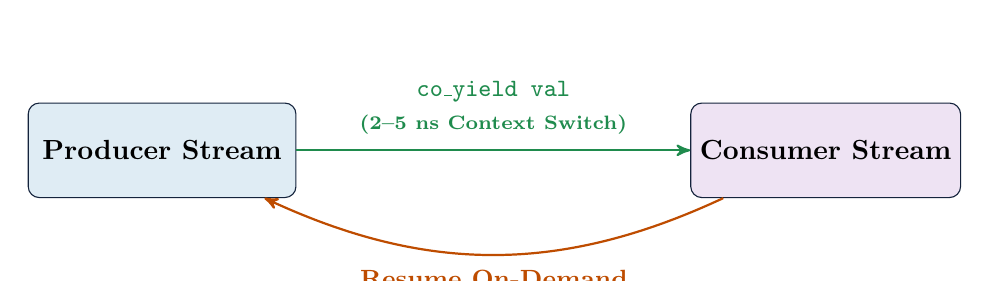
\begin{tikzpicture}[node distance=5.0cm, auto, >=stealth']
    \node [draw=sisalnavy, rounded corners=4pt, rectangle, fill=sisalblue!15, minimum width=3.4cm, minimum height=1.2cm, align=center, font=\bfseries] (producer) {Producer Stream};
    \node [draw=sisalnavy, rounded corners=4pt, rectangle, fill=sisalpurple!15, minimum width=3.4cm, minimum height=1.2cm, align=center, font=\bfseries, right=5.0cm of producer] (consumer) {Consumer Stream};
    
    \draw [->, thick, sisalgreen!80!black] (producer) -- node[above=2pt, font=\small\bfseries, align=center] {\texttt{co\_yield val}\\[1pt]\scriptsize (2--5 ns Context Switch)} (consumer);
    \draw [->, thick, sisalorange!90!black] (consumer) to[bend left=25] node[below=2pt, font=\small\bfseries] {Resume On-Demand} (producer);
\end{tikzpicture}
\caption{Zero-Allocation Coroutine Stream Switching.}
\label{fig:coroutine_switch}
\end{figure}

\begin{lstlisting}[caption={Stream Generator Function}]
function GenerateIntegers( start, limit : integer returns stream[integer] )
  for initial
    val := start
  while val <= limit repeat
    val := old val + 1
  returns
    stream of val
  end for
end function
\end{lstlisting}

\section{Heap Allocation Elision (HALO) Performance}
Because C++20 coroutine frames fit within standard frame boundaries when inlined, modern compilers (GCC 13+, Clang 16+) perform Heap Allocation Elision Optimization (HALO). This places coroutine frame state directly on the caller stack frame, achieving:
\begin{itemize}
    \item \textbf{Context Switch Overhead}: 2 to 5 nanoseconds (30$\times$--100$\times$ faster than POSIX \texttt{ucontext} or OS thread context switches).
    \item \textbf{Memory Overhead}: Zero heap allocation overhead for stream pipelines.
\end{itemize}

\chapter{Side-Effect Monad Ordering}
\label{chap:side_effects_monads}

\section{Reconciling Pure Functional Dataflow with I/O}
Pure dataflow languages traditionally struggle with imperative I/O operations. In a pure dataflow graph (such as Sisal 1.2), node execution is driven strictly by data dependencies: a node executes as soon as all of its input arguments become available. When sub-expressions have no data dependencies between them, they are scheduled concurrently across available processor threads or executed in arbitrary order.

While this non-deterministic out-of-order execution model is ideal for high-performance data parallelism, it presents severe challenges for practical programming tasks:
\begin{itemize}
    \item \textbf{Console Output Interleaving}: Concurrent printing from multiple parallel sub-graph branches causes character streams to collide and interleave unpredictably.
    \item \textbf{Debug Tracing}: Programmers cannot easily trace algorithm iteration steps or log intermediate values when execution timing varies between runs.
    \item \textbf{Sequential File/Stream Access}: Operations like writing consecutive record chunks to stdout or disk files require a guaranteed, deterministic order.
\end{itemize}

Sisal-2026 solves this challenge by introducing \textbf{Monad Control Ports} into the compiler's IF1 intermediate representation graph.

\section{What is a Monad in Sisal-2026?}
In functional programming and category theory, a \emph{monad} is a design pattern that structures computations by encapsulating value evaluation alongside side-effect execution contexts. In Sisal-2026, a monad represents an implicit, linearly-threaded sequencing state that enforces a strict execution order between side-effecting operations without violating the language's core single-assignment immutability rules.

Conceptually, a side-effecting built-in function in Sisal-2026 operates as a state-transformer monad:
\begin{equation}
f :: A \to S \to (B, S)
\end{equation}
where $A$ is the input argument, $B$ is the returned result value, and $S$ represents an abstract "World State" token. Rather than exposing state tokens to the programmer, the compiler automatically threads this state token through side-effecting operations, creating an explicit linear execution sequence.

\section{Serialization \& Imperative Style for Practical Scenarios}
To handle practical software engineering requirements—such as progress logging, error reporting, and stream output—Sisal-2026 enables developers to write familiar, imperative-style sequential code within pure functional routines.

When a developer writes consecutive side-effecting statements:
\begin{lstlisting}[caption={Imperative-Style Logging Sequence in Sisal-2026}]
function ExecutePipeline( data : array_dv[double] returns array_dv[double] )
  let
    _ := printf("Phase 1: Starting computation...\n");
    R1 := ProcessPhase1(data);
    _ := printf("Phase 2: Intermediate processing complete.\n");
    R2 := ProcessPhase2(R1);
    _ := printf("Phase 3: Finalizing results.\n")
  in
    R2
  end let
end function
\end{lstlisting}

Sisal-2026 reconciles this imperative notation with its dataflow engine through \textbf{deterministic serialization}:
\begin{enumerate}
    \item \textbf{Localized Imperative Sequencing}: Side-effecting statements are executed in exact lexicographic (source file) order.
    \item \textbf{Concurrent Functional Subgraphs}: Pure mathematical expressions (\texttt{ProcessPhase1}, \texttt{ProcessPhase2}, array arithmetic) continue to execute with maximum data parallelism across all available CPU worker threads.
    \item \textbf{No Non-Deterministic Race Conditions}: Output buffers are never corrupted by out-of-order thread scheduling.
\end{enumerate}

\section{Monad Control Ports in the IF1 Intermediate Representation}
A \textbf{Monad Control Port} is a compiler-inserted IR graph port designed to carry sequence control tokens. When the Sisal-2026 parser encounters side-effecting built-in procedures (\texttt{printf}, \texttt{cout}, \texttt{cerr}), it decorates the corresponding IF1 AST nodes with dedicated monad ports:
\begin{itemize}
    \item \texttt{PRINTF\_TY}: Monad sequence control port for standard output logging.
    \item \texttt{COUT\_TY}: C++ stream output monad sequence port.
    \item \texttt{CERR\_TY}: Standard error stream monad sequence port.
\end{itemize}

During graph lowering, the compiler constructs artificial control-dependency edges (\emph{Monad Control Edges}) between consecutive side-effecting nodes based on their program text position. An IF1 node possessing an incoming Monad Control Edge is prohibited from firing until the predecessor side-effecting node has completed execution and emitted its control token.

\begin{figure}[h!]
\centering
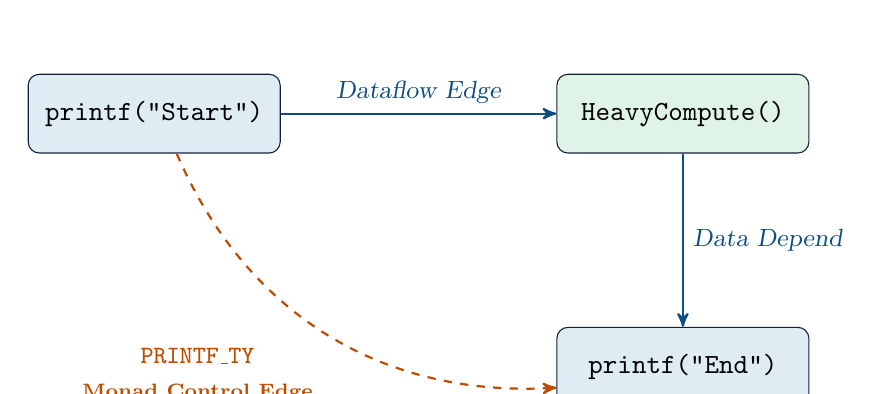
\begin{tikzpicture}[node distance=2.2cm, auto, >=stealth']
    % Nodes
    \node [draw=sisalnavy, rounded corners=4pt, rectangle, fill=sisalblue!15, minimum width=3.2cm, minimum height=1.0cm, align=center, font=\bfseries] (p1) {\texttt{printf("Start")}};
    \node [draw=sisalnavy, rounded corners=4pt, rectangle, fill=sisalgreen!15, minimum width=3.2cm, minimum height=1.0cm, align=center, font=\bfseries, right=3.5cm of p1] (compute) {\texttt{HeavyCompute()}};
    \node [draw=sisalnavy, rounded corners=4pt, rectangle, fill=sisalblue!15, minimum width=3.2cm, minimum height=1.0cm, align=center, font=\bfseries, below=2.2cm of compute] (p2) {\texttt{printf("End")}};
    
    % Dataflow Edges (Pure Computation Path)
    \draw [->, thick, sisaldarkblue] (p1) -- node[above, font=\small\slshape] {Dataflow Edge} (compute);
    \draw [->, thick, sisaldarkblue] (compute) -- node[right, font=\small\slshape] {Data Depend} (p2);
    
    % Monad Sequencing Control Edge (Curved to prevent box collision)
    \draw [->, thick, sisalorange!90!black, dashed] (p1) to[bend right=35] node[below left=2pt, font=\small\bfseries, align=center] {\texttt{PRINTF\_TY}\\[1pt]\scriptsize Monad Control Edge} (p2);
\end{tikzpicture}
\caption{Monad Control Port Dependency Edge in IF1 Graph.}
\label{fig:monad_port}
\end{figure}

As illustrated in Figure~\ref{fig:monad_port}, pure computation paths (\texttt{HeavyCompute()}) execute asynchronously according to data availability, while side-effecting nodes are linked via the dashed \texttt{PRINTF\_TY} Monad Control Edge to guarantee strict ordering.

\section{Value Pass-Through vs. Wildcard Idioms}
Sisal-2026 supports two primary statement idioms for \texttt{printf} logging:
\begin{itemize}
    \item \textbf{Wildcard Binding (\texttt{\_ := printf(...)})}: Evaluates the formatted logging statement and discards the return value using the wildcard pattern \texttt{\_}. This pattern is ideal for stand-alone progress messages.
    \item \textbf{Value Pass-Through (\texttt{res := printf("\%d\textbackslash n", val)})}: Logs the formatted message while transparently evaluating and returning the printed value argument. This permits inline debug logging without disrupting dataflow or polluting the program with temporary variable declarations.
\end{itemize}

\section{Deterministic Lexicographic Ordering Guarantees}
By combining Monad Control Ports in the IR with single-assignment language semantics, Sisal-2026 achieves a powerful synthesis:
\begin{enumerate}
    \item \textbf{Guaranteed Determinism}: Given identical inputs, a Sisal-2026 program will produce the exact same console log output in the exact same sequence across every run, regardless of hardware core count or thread scheduling order.
    \item \textbf{Zero Impact on Pure Parallelism}: Monad control edges sequence only nodes decorated with side-effect ports. Independent mathematical operations, array contractions, tensor operations, and loop iterations remain 100\% parallelizable across multicore targets.
\end{enumerate}

\chapter{The IF1 Intermediate Representation}
\label{chap:if1_ir}

\section{IF1 Dataflow Graph Architecture}
The core intermediate representation of the Sisal-2026 compiler is \textbf{IF1} (\emph{Intermediate Format 1}), an acyclic directed dataflow graph format.

An IF1 graph consists of:
\begin{itemize}
    \item \textbf{Nodes}: Representing operations, function calls, or subgraphs.
    \item \textbf{Edges}: Representing data values flowing from output ports of source nodes to input ports of destination nodes.
    \item \textbf{Types}: Attached to every edge to enforce type safety.
\end{itemize}

\section{Simple vs. Compound Nodes}
IF1 distinguishes between two primary categories of nodes:
\begin{enumerate}
    \item \textbf{Simple Nodes}: Primitive scalar arithmetic, dope vector indexing, logic, or function calls (e.g. \texttt{Plus}, \texttt{Times}, \texttt{DopeVectorSlice}).
    \item \textbf{Compound Nodes}: Complex control structures containing nested subgraphs (e.g. \texttt{SelectNode} for conditionals, \texttt{ForallNode} for parallel loops, \texttt{LoopANode}/\texttt{LoopBNode} for sequential loops).
\end{enumerate}

\begin{figure}[h!]
\centering
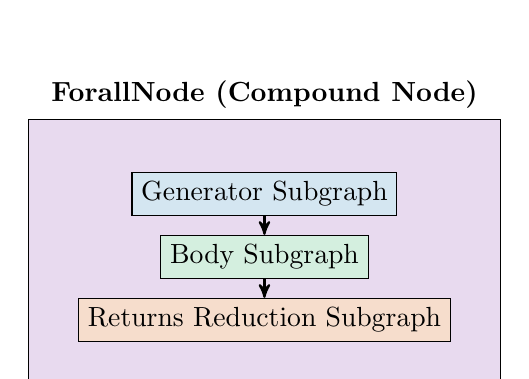
\begin{tikzpicture}[node distance=1.5cm, auto, >=stealth']
    \node [draw, rectangle, fill=sisalpurple!20, minimum width=6cm, minimum height=3.5cm, label=above:\textbf{ForallNode (Compound Node)}] (forall) {};
    
    \node [draw, rectangle, fill=sisalblue!20, yshift=0.8cm] (gen) at (forall.center) {Generator Subgraph};
    \node [draw, rectangle, fill=sisalgreen!20] (body) at (forall.center) {Body Subgraph};
    \node [draw, rectangle, fill=sisalorange!20, yshift=-0.8cm] (ret) at (forall.center) {Returns Reduction Subgraph};
    
    \draw [->, thick] (gen) -- (body);
    \draw [->, thick] (body) -- (ret);
\end{tikzpicture}
\caption{Structure of an IF1 Compound \texttt{ForallNode}.}
\label{fig:if1_compound}
\end{figure}

\section{Optimization Passes}
The Sisal-2026 compiler executes several optimization passes directly on IF1 graphs:
\begin{itemize}
    \item \textbf{Common Subexpression Elimination (CSE)}: Merges identical pure subgraphs.
    \item \textbf{Dead Code Elimination (DCE)}: Removes unreferenced node outputs.
    \item \textbf{Loop Invariant Code Motion (LICM)}: Hoists constant expressions out of sequential loops.
    \item \textbf{Copy Elimination \& Static Liveness}: Eliminates array buffer copies whenever reference counts equal 1.
\end{itemize}

\chapter{C++23 Runtime Architecture}
\label{chap:cpp23_runtime}

\section{\texttt{sisal\_runtime.h} Execution Engine}
The Sisal-2026 code generator targets modern C++23. The runtime layer is implemented in \texttt{runtime/sisal\_runtime.h} and provides header-only execution primitives for dope vectors, parallel loops, SIMD intrinsics, and BLAS routines.

\section{Memory Management \& Reference Counting}
Memory allocation for \texttt{array\_dv} elements is managed via aligned heap allocators. Reference counting operates on the dope vector metadata:

\begin{lstlisting}[caption={Dope Vector Reference Counting API}]
inline sisal_array_t* sisal_dv_retain(sisal_array_t* arr) {
    if (arr) {
        arr->ref_count++;
    }
    return arr;
}

inline void sisal_dv_release(sisal_array_t* arr) {
    if (arr && --(arr->ref_count) == 0) {
        aligned_free(arr->data);
        free(arr->shape);
        free(arr->stride);
        free(arr);
    }
}
\end{lstlisting}

\section{Hardware BLAS \& LAPACK Integration}
For matrix-matrix and matrix-vector operations generated by \texttt{EINSUM} or bulk primitives, the runtime interfaces with hardware-accelerated BLAS libraries (Apple Accelerate framework on macOS, OpenBLAS / MKL on Linux):

\begin{lstlisting}[caption={BLAS DGEMM Invocation in C++23 Runtime}]
inline sisal_array_t* sisal_dv_matmul(sisal_array_t* A, sisal_array_t* B) {
    % Verify rank-2 compatibility and stride alignment
    int M = A->shape[0];
    int K = A->shape[1];
    int N = B->shape[1];
    
    sisal_array_t* C = sisal_dv_alloc_2d(M, N, sizeof(double));
    
    cblas_dgemm(CblasRowMajor, CblasNoTrans, CblasNoTrans,
                M, N, K, 1.0,
                (const double*)A->data, A->stride[0],
                (const double*)B->data, B->stride[0],
                0.0, (double*)C->data, C->stride[0]);
                
    return C;
}
\end{lstlisting}

\chapter{Copy Elimination, Liveness Analysis \& Memory Reuse}
\label{chap:copy_enforcement}

\section{The Single-Assignment Memory Challenge}
A foundational principle of pure functional dataflow languages is \emph{single assignment}: once an array variable is bound, its contents are mathematically immutable. However, naive enforcement of immutability would require generating a full $O(N)$ deep memory copy (\texttt{memcpy}) whenever an array element or slice is modified (e.g., $A' = A[i \gets v]$). In large-scale scientific computation involving multi-gigabyte matrices, such redundant copying would degrade performance and destroy cache locality.

Historically, Sisal~1.2 and 2.0 addressed this challenge using pure compile-time optimizations known as \emph{build-in-place} and \emph{update-in-place} passes. While effective for simple loops, purely static passes conservatively fall back to full memory copies whenever complex control flow, recursion, or dynamic aliasing prevents proving at compile time that live ranges are non-overlapping.

\textbf{Sisal-2026} introduces a hybrid static-dynamic memory architecture:
\begin{enumerate}
    \item \textbf{Static Edge Liveness Analysis}: A compiler optimization pass computes topological liveness across dataflow graph edges, identifying the \emph{topologically last consumer} of every array reference and emitting ownership-stealing directives.
    \item \textbf{Dynamic Copy-on-Write (CoW) Reference Counting}: A C++23 runtime system tracks array buffer reference counts (\texttt{ref\_count}). When an array update is executed, if the reference count is $1$ (guaranteed by the static pass on the last consumer edge), the update executes \textbf{in-place} with zero memory allocation. If the reference count exceeds $1$ (due to concurrent live branches), the runtime dynamically intercepts the update and performs a Copy-on-Write allocation.
\end{enumerate}

\section{Static Edge Liveness Analysis in the Compiler}
In Sisal-2026, the compiler backend (\texttt{src/backend/cpp/cpp\_lower.ml}) implements static edge liveness analysis via \texttt{scan\_edge\_liveness}. 

Given an IF1 dataflow graph $G = (V, E)$, every node $n \in V$ represents a primitive computation or compound control-flow construct, and every edge $e = ((n_{src}, p_{src}), (n_{dst}, p_{dst})) \in E$ represents a directed value dependency.

For a produced array value at output port $(n_{src}, p_{src})$, let $C(n_{src}, p_{src})$ denote the set of all consumer edges reading that value:
\begin{equation}
C(n_{src}, p_{src}) = \{ ((n_{src}, p_{src}), (n_{dst}, p_{dst})) \in E \}
\end{equation}

The compiler computes a topological sorting $T : V \to \mathbb{N}$ of all graph nodes. The \emph{topologically last consumer edge} $e_{last} \in C(n_{src}, p_{src})$ is defined as:
\begin{equation}
e_{last} = \arg\max_{((n_{src}, p_{src}), (n_{dst}, p_{dst})) \in C(n_{src}, p_{src})} T(n_{dst})
\end{equation}

On $e_{last}$, the static analysis pass tags the edge in \texttt{edge\_free\_map}. During C++ code generation, the backend emits ownership-stealing instructions (such as \texttt{std::move} or passing a mutable reference \texttt{\&A}) for $e_{last}$, while emitting reference-incrementing code for all earlier consumer edges.

\section{Static Liveness \& Memory Ownership Algorithm}
Algorithm~\ref{alg:liveness_cow} presents the formal algorithm for static edge liveness analysis and ownership assignment as implemented in the Sisal-2026 compiler backend.

\begin{algorithm}[H]
\caption{Static Edge Liveness Analysis \& Memory Ownership Pass}
\label{alg:liveness_cow}
\begin{algorithmic}[1]
\REQUIRE IF1 Dataflow Subgraph $G = (V, E)$, Port Map $M$, Typemap $TM$
\ENSURE Edge Free Map $EFM$ mapping last consumer edges to release directives

\STATE \COMMENT{\textbf{Step 1: Compute Topological Node Ordering}}
\STATE $L \gets \text{TopoSort}(V, E)$
\STATE $\text{TopoPos} \gets \text{EmptyMap}()$
\FORALL{node $v \in L$ at index $i$}
    \STATE $\text{TopoPos}[v] \gets i$
\ENDFOR

\STATE \COMMENT{\textbf{Step 2: Group Consumer Edges by Producer Output Port}}
\STATE $\text{Consumers} \gets \text{EmptyMap}()$
\FORALL{edge $e = ((n_{src}, p_{src}), (n_{dst}, p_{dst}), \text{type}) \in E$}
    \STATE $\text{Key} \gets (n_{src}, p_{src})$
    \STATE $\text{Consumers}[\text{Key}] \gets \text{Consumers}[\text{Key}] \cup \{ e \}$
\ENDFOR

\STATE \COMMENT{\textbf{Step 3: Identify Topologically Last Consumer Edge}}
\FORALL{Key $(n_{src}, p_{src}) \in \text{Keys}(\text{Consumers})$}
    \STATE $\text{EdgeList} \gets \text{Consumers}[(n_{src}, p_{src})]$
    \STATE Sort $\text{EdgeList}$ ascending by $\text{TopoPos}[n_{dst}]$
    \STATE $e_{last} \gets \text{LastElement}(\text{EdgeList})$
    \STATE Let $e_{last} = ((n_{src}, p_{src}), (n_{dst}, p_{dst}), \text{type})$
    \STATE $EFM[(n_{src}, p_{src}, n_{dst}, p_{dst})] \gets \text{STOLEN\_OWNERSHIP}$
\ENDFOR

\STATE \COMMENT{\textbf{Step 4: Code Generation Lowering}}
\FORALL{edge $e = ((n_{src}, p_{src}), (n_{dst}, p_{dst})) \in E$}
    \IF{$EFM[e] == \text{STOLEN\_OWNERSHIP}$}
        \STATE Emit \texttt{std::move(var\_src)} or pass \texttt{\&var\_src} (Steal buffer, decrement $\text{ref\_count}$)
    \ELSE
        \STATE Emit \texttt{var\_src} (Copy handle, increment $\text{ref\_count}$)
    \ENDIF
\ENDFOR
\RETURN $EFM$
\end{algorithmic}
\end{algorithm}

\section{Dynamic Copy-on-Write (CoW) Runtime Architecture}
The runtime system complements the static compiler pass by managing array dope vectors (\texttt{sisal\_array\_t}) and checking reference counts at execution time.

\begin{figure}[h!]
\centering
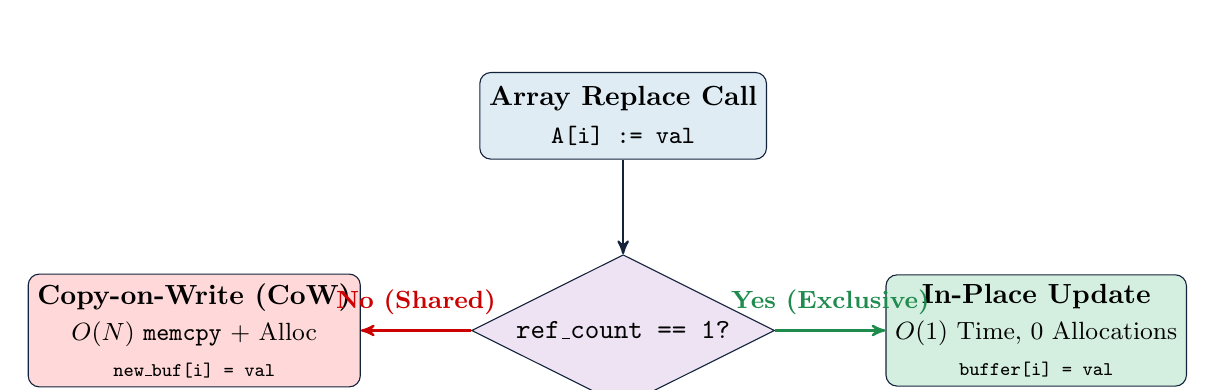
\begin{tikzpicture}[node distance=1.8cm, auto, >=stealth']
    \node [draw=sisalnavy, rectangle, fill=sisalblue!15, rounded corners=4pt, align=center, minimum width=3.4cm, minimum height=1.1cm, font=\bfseries] (replace) {\textbf{Array Replace Call}\\[2pt]\texttt{\small A[i] := val}};
    \node [draw=sisalnavy, diamond, fill=sisalpurple!15, aspect=2, align=center, font=\bfseries, below=1.2cm of replace] (check) {\texttt{ref\_count == 1?}};
    
    \node [draw=sisalnavy, rectangle, fill=sisalgreen!20, rounded corners=4pt, align=center, minimum width=3.4cm, minimum height=1.2cm, right=1.4cm of check] (inplace) {\textbf{In-Place Update}\\[1pt]\small $O(1)$ Time, 0 Allocations\\[1pt]\texttt{\scriptsize buffer[i] = val}};
    \node [draw=sisalnavy, rectangle, fill=red!15, rounded corners=4pt, align=center, minimum width=3.4cm, minimum height=1.2cm, left=1.4cm of check] (cow) {\textbf{Copy-on-Write (CoW)}\\[1pt]\small $O(N)$ \texttt{memcpy} + Alloc\\[1pt]\texttt{\scriptsize new\_buf[i] = val}};
    
    \draw [->, thick, sisalnavy] (replace) -- (check);
    \draw [->, thick, sisalgreen!80!black] (check) -- node [above=2pt, font=\small\bfseries] {Yes (Exclusive)} (inplace);
    \draw [->, thick, red!80!black] (check) -- node [above=2pt, font=\small\bfseries] {No (Shared)} (cow);
\end{tikzpicture}
\caption{Decision Flowchart for Sisal-2026 Copy-on-Write (CoW) Runtime.}
\label{fig:cow_flowchart}
\end{figure}

Every array value \texttt{sisal\_array\_t} maintains reference counting over its underlying contiguous memory buffer. When an array modification function (e.g., \texttt{sisal\_array\_replace\_i32}) is invoked, the runtime executes the logic shown in Listing~\ref{lst:cow_runtime}.

\begin{lstlisting}[language=C++,caption={Sisal-2026 Copy-on-Write Replacement Runtime Logic},label=lst:cow_runtime]
sisal_array_t sisal_array_consume_replace(sisal_array_t* arr_ptr, 
                                           size_t index, 
                                           float val) {
    sisal_array_t result;
    // Steal reference from caller
    result.data = std::move(arr_ptr->data); 
    result.size = arr_ptr->size;
    
    // Check reference count on underlying buffer
    if (result.data.use_count() > 1) {
        // Shared ownership: Copy-on-Write (CoW) required!
        void* new_ptr = NULL;
        posix_memalign(&new_ptr, 4096, result.size * sizeof(float));
        memcpy(new_ptr, result.data.get(), result.size * sizeof(float));
        result.data = std::shared_ptr<float>((float*)new_ptr, FreeDeleter());
    } else {
        // Exclusive ownership (use_count == 1): In-place update!
    }
    
    result.data.get()[index] = val;
    return result;
}
\end{lstlisting}

\section{Empirical Analysis of Test Cases}
To verify the hybrid static-dynamic memory model, the Sisal-2026 test suite contains dedicated regression programs and unit tests.

\subsection{Case 1: Overlapping Live Ranges (\texttt{array\_copy\_liveness\_dv.sis})}
The test program \texttt{array\_copy\_liveness\_dv.sis} forces overlapping live ranges where two array bindings remain live simultaneously.

\begin{lstlisting}[caption={Sisal Source: \texttt{array\_copy\_liveness\_dv.sis}}]
function Main( returns array_dv[integer], array_dv[integer] )
  let
    A := array_dv [1: 10, 20, 30];
    B := A;
    B2 := B[1: 999]
  in
    A, B2
  end let
end function
\end{lstlisting}

\subsubsection{Compiler Analysis \& Execution Trace}
\begin{itemize}
    \item \textbf{Static Graph Analysis}: The compiler detects that array \texttt{A} is returned directly as output 0 (\texttt{returns A}) AND used to define \texttt{B}. Because \texttt{A} has multiple active output edges, \texttt{scan\_edge\_liveness} cannot mark \texttt{A} as dead.
    \item \textbf{Runtime Execution}: \texttt{B := A} increments the reference count of the underlying buffer to $\text{ref\_count} = 2$.
    \item \textbf{CoW Interception}: When \texttt{B2 := B[1: 999]} executes, the runtime checks $\text{ref\_count} = 2 > 1$, intercepts the write, allocates a new 3-element buffer, and copies \texttt{[10, 20, 30]} into \texttt{B2}.
    \item \textbf{C++ Assertion Verification}: In \texttt{test/e2e/parts/dv\_part\_01.cpp}, the test runner confirms:
    \begin{lstlisting}[language=C++]
    check("A remains [10, 20, 30]", A.data.get()[0] == 10);
    check("B2 modified to [999, 20, 30]", B2.data.get()[0] == 999);
    check("A and B2 have separate data buffers", A.data != B2.data);
    \end{lstlisting}
\end{itemize}

\subsection{Case 2: Non-Overlapping Live Ranges (Sequential Loop Updates)}
In contrast, consider a sequential loop performing iterative element replacement:

\begin{lstlisting}[caption={Sisal Source: In-Place Loop Update}]
function InPlaceLoop( N : integer returns array_dv[integer] )
  for initial
    i := 1;
    A := array_dv [1: 10, 20, 30, 40, 50];
  while i <= 5 repeat
    i := old i + 1;
    A := (old A)[old i: (old i) * 10];
  returns value of A
  end for
end function
\end{lstlisting}

\subsubsection{Compiler Analysis \& Execution Trace}
\begin{itemize}
    \item \textbf{Static Graph Analysis}: In each loop iteration, \texttt{old A} has exactly one consumer: the element replacement node. \texttt{scan\_edge\_liveness} identifies this edge as the topologically last consumer edge, tagging it for ownership stealing.
    \item \textbf{Compiler Code Generation}: The compiler generates code that passes \texttt{\&A} (stealing \texttt{old A}'s pointer and releasing the previous binding reference).
    \item \textbf{Runtime Execution}: When the replacement helper checks $\text{ref\_count}$, it discovers $\text{ref\_count} = 1$. The update executes \textbf{in-place} directly into the memory buffer.
    \item \textbf{Performance}: All 5 loop iterations execute in $O(1)$ space with zero memory allocation and zero \texttt{memcpy} calls.
\end{itemize}

\section{Summary of Memory Enforcement Rules}
Table~\ref{tab:copy_summary} summarizes the interaction between static compiler passes and dynamic runtime mechanisms across common Sisal-2026 coding patterns.

\begin{table}[h!]
\centering
\caption{Summary of Copy Enforcement across Sisal-2026 Coding Patterns}
\label{tab:copy_summary}
\begin{tabularx}{\textwidth}{X p{3.2cm} p{3.2cm} X}
\toprule
\textbf{Sisal Coding Pattern} & \textbf{Static Compiler Action} & \textbf{Runtime Action} & \textbf{Memory \& Time Performance} \\
\midrule
Sequential Loop Update (\texttt{A := (old A)[i: v]}) & \texttt{scan\_edge\_liveness} marks input dead; steals ownership. & Sees $\text{ref\_count} = 1$; updates in-place. & $O(1)$ Space, $0$ Allocations, $0$ \texttt{memcpy}. \\
\midrule
Zero-Copy Slice (\texttt{Sub = M[1..2, 3..4]}) & Shifts dope vector origin/strides metadata. & Shares buffer; increments $\text{ref\_count}$. & $O(1)$ Constant Time Metadata View. \\
\midrule
Aliased Modification (\texttt{B := A; B2 := B[i: v]}) & Detects active live branch on \texttt{A}; retains reference. & Sees $\text{ref\_count} > 1$; triggers CoW. & $O(N)$ Duplicated Buffer Allocation \& Copy. \\
\bottomrule
\end{tabularx}
\end{table}

\chapter{Modern Neural Network Architectures: Deep Dive into the Sisal-2026 Transformer Graph}
\label{chap:transformer_architecture}

Modern Large Language Models (LLMs) rely on highly structured tensor transformation graphs composed of linear projections, point-wise non-linearities, non-local attention contractions, and normalization layers. While imperative frameworks often struggle with manual memory management, activation caching, and explicit execution scheduling, functional dataflow languages represent these architectures as pure, single-assignment Directed Acyclic Graphs (DAGs).

In \textbf{Sisal-2026}, modern Transformer blocks---specifically featuring \textbf{Root-Mean-Square Layer Normalization (RMSNorm)}, \textbf{Grouped Query Attention (GQA)}, \textbf{SwiGLU Gated Feed-Forward Networks (FFN)}, and \textbf{Residual Connections}---are expressed natively as high-level dataflow programs by combining rank-polymorphic whole-array primitives with modern Einstein summation (\texttt{EINSUM}) syntax. This chapter provides a comprehensive, operator-by-operator deep dive into the Transformer graph in Sisal-2026, analyzing the mathematical formulation, high-level Sisal syntax, IF1 Intermediate Representation, C++23 runtime lowering, and zero-copy buffer optimizations for every single component.

\section{System Architecture \& Functional Pipeline}
\label{sec:transformer_pipeline}

The Transformer layer consumes an input activation tensor $X \in \mathbb{R}^{B \times S \times D}$, where $B$ is the batch size, $S$ is the sequence length, and $D$ is the hidden dimension. The layer processes $X$ through two main sub-blocks (Attention and Feed-Forward), each preceded by pre-normalization (RMSNorm) and bound by additive residual connections.

Figure~\ref{fig:transformer_dag} illustrates the complete dataflow graph within Sisal-2026.

\begin{figure}[htbp]
\centering
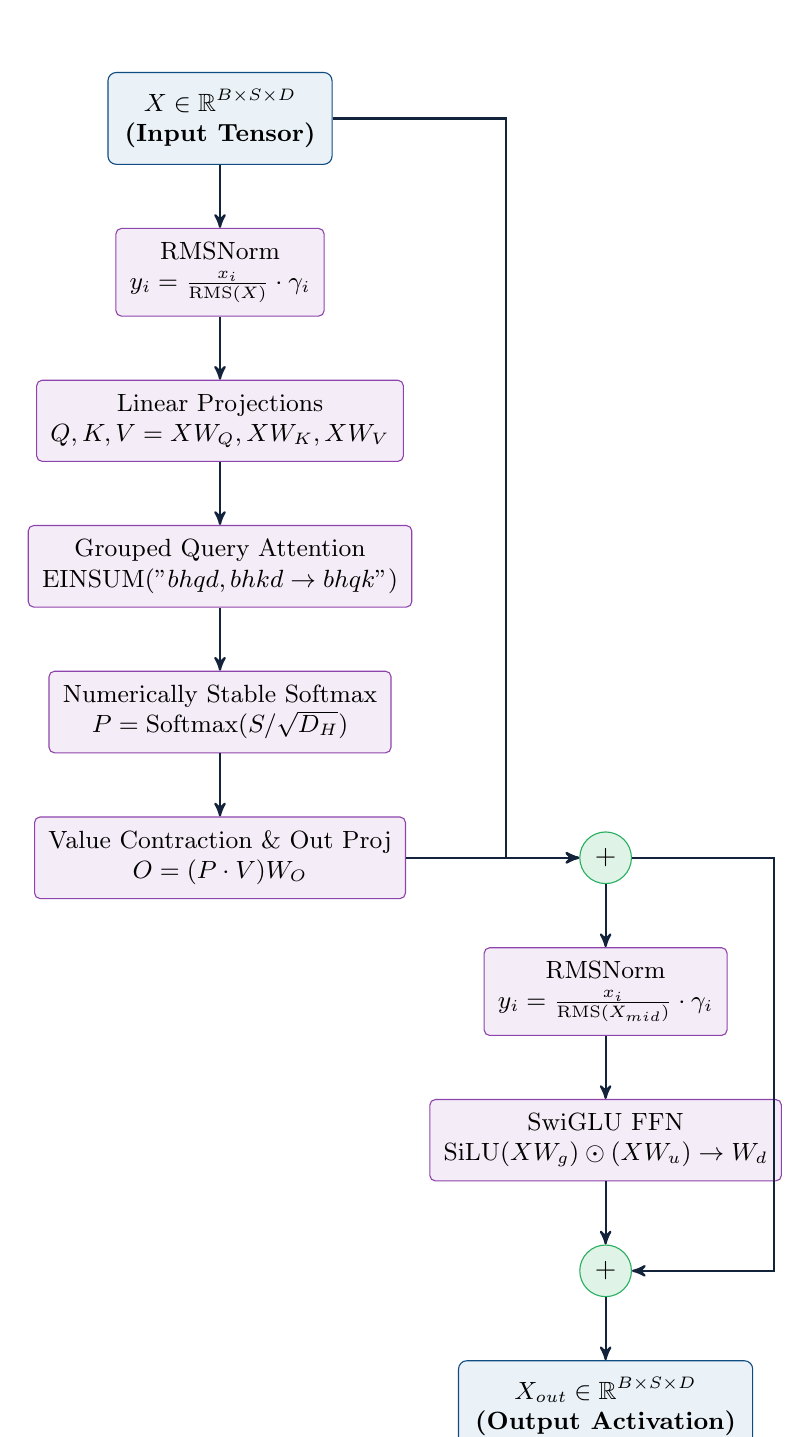
\begin{tikzpicture}[node distance=1.2cm and 1.8cm, auto, >=stealth',
  block/.style={draw=sisaldarkblue, fill=sisalblue!10, rectangle, rounded corners=3pt, inner sep=6pt, align=center, font=\small\bfseries},
  op/.style={draw=sisalpurple, fill=sisalpurple!10, rectangle, rounded corners=2pt, inner sep=5pt, align=center, font=\small},
  add/.style={draw=sisalgreen, fill=sisalgreen!15, circle, inner sep=3pt, font=\bfseries},
  line/.style={draw=sisalnavy, ->, thick}
]

  % Input Node
  \node [block] (input) {$X \in \mathbb{R}^{B \times S \times D}$ \\ (Input Tensor)};

  % Attention Path
  \node [op, below=0.8cm of input] (rms1) {RMSNorm \\ $y_i = \frac{x_i}{\text{RMS}(X)} \cdot \gamma_i$};
  \node [op, below=0.8cm of rms1] (qkv) {Linear Projections \\ $Q, K, V = X W_Q, X W_K, X W_V$};
  \node [op, below=0.8cm of qkv] (gqa) {Grouped Query Attention \\ $\text{EINSUM}("bhqd,bhkd \to bhqk")$};
  \node [op, below=0.8cm of gqa] (softmax) {Numerically Stable Softmax \\ $P = \text{Softmax}(S / \sqrt{D_H})$};
  \node [op, below=0.8cm of softmax] (out_proj) {Value Contraction \& Out Proj \\ $O = (P \cdot V) W_O$};
  
  % First Residual Add
  \node [add, right=2.2cm of out_proj] (add1) {$+$};

  % FFN Path
  \node [op, below=0.8cm of add1] (rms2) {RMSNorm \\ $y_i = \frac{x_i}{\text{RMS}(X_{mid})} \cdot \gamma_i$};
  \node [op, below=0.8cm of rms2] (swiglu) {SwiGLU FFN \\ $\text{SiLU}(X W_g) \odot (X W_u) \to W_d$};
  
  % Second Residual Add
  \node [add, below=0.8cm of swiglu] (add2) {$+$};
  \node [block, below=0.8cm of add2] (output) {$X_{out} \in \mathbb{R}^{B \times S \times D}$ \\ (Output Activation)};

  % Flow Connections
  \draw [line] (input) -- (rms1);
  \draw [line] (rms1) -- (qkv);
  \draw [line] (qkv) -- (gqa);
  \draw [line] (gqa) -- (softmax);
  \draw [line] (softmax) -- (out_proj);
  \draw [line] (out_proj) -- (add1);

  % Residual 1 Bypass
  \draw [line] (input.east) -- ++(2.2,0) |- (add1);

  % FFN Flow
  \draw [line] (add1) -- (rms2);
  \draw [line] (rms2) -- (swiglu);
  \draw [line] (swiglu) -- (add2);

  % Residual 2 Bypass
  \draw [line] (add1.east) -- ++(1.8,0) |- (add2);
  \draw [line] (add2) -- (output);

\end{tikzpicture}
\caption{Complete Single-Assignment Dataflow DAG for a Modern Transformer Block in Sisal-2026.}
\label{fig:transformer_dag}
\end{figure}

\section{Complete Annotated Sisal-2026 Source Code}
\label{sec:transformer_code}

The complete implementation of the GQA SwiGLU Transformer layer in Sisal-2026 is shown in Listing~\ref{lst:transformer_full}.

\begin{lstlisting}[language=Sisal, caption={Sisal-2026 Transformer Block Implementation (\texttt{transformer\_gqa\_swiglu.sis}).}, label={lst:transformer_full}]
% Sisal-2026 Modern Transformer Layer (RMSNorm, GQA, SwiGLU, Residuals)

function RMSNorm( X : array_dv[double]; Gamma : array_dv[double]; eps : double 
                  returns array_dv[double] )
  let
    Variance := MEAN(X * X);
    Scale := 1.0d0 / SQRT(Variance + eps)
  in
    X * Scale * Gamma
  end let
end function

function Swish( X : array_dv[double] returns array_dv[double] )
  % Pointwise SiLU / Swish activation
  X / (1.0d0 + EXP(-X))
end function

function SwiGLUFFN( X : array_dv[double]; W1 : array_dv[double]; 
                    W2 : array_dv[double]; W3 : array_dv[double] 
                    returns array_dv[double] )
  let
    % Note: MATMUL(X, W1) or EINSUM("sd,dh->sh", X, W1) are interchangeable for 2D matrices
    Gate := EINSUM("sd,dh->sh", X, W1);
    Up   := EINSUM("sd,dh->sh", X, W2);
    SwishGate := Swish(Gate);
    
    % Direct elementwise Hadamard product
    Hidden := SwishGate * Up
  in
    EINSUM("sh,hd->sd", Hidden, W3)
  end let
end function

function Softmax( X : array_dv[double] returns array_dv[double] )
  let
    Rows := array_size(X)
  in
    for i in 1, Rows
      RowMax := GREATEST(X[i, ..]);
      ExpRow := EXP(X[i, ..] - RowMax);
      SumExp := SUM(ExpRow)
    returns array_dv of ExpRow / SumExp
    end for
  end let
end function

function GQAttention( Q : array_dv[double]; K : array_dv[double]; 
                       V : array_dv[double]; W_O : array_dv[double]; 
                       scale : double returns array_dv[double] )
  let
    % 1. Compute multi-head attention scores Q * K^T and scale
    % Note: MATMUL, INNERPRODUCT, or EINSUM may be used for matrix products
    Scores := MATMUL(Q, K) * scale;
    KeyLen := array_size(V);
    
    % 2. Softmax normalization across key sequence axis
    AttnWeights := Softmax(Scores, KeyLen);
    
    % 3. Aggregate values AttnWeights * V via MATMUL / INNERPRODUCT
    Context := MATMUL(AttnWeights, V);
    
    % 4. Output projection to model dimension
    Out := MATMUL(Context, W_O)
  in
    Out
  end let
end function

function TransformerBlock( X : array_dv[double]; 
                          Q : array_dv[double]; K : array_dv[double]; 
                          V : array_dv[double]; W_O : array_dv[double];
                          W1 : array_dv[double]; W2 : array_dv[double]; 
                          W3 : array_dv[double]; Gamma1 : array_dv[double]; 
                          Gamma2 : array_dv[double]; scale, eps : double 
                          returns array_dv[double] )
  let
    % Pre-LayerNorm 1 + Self-Attention + Residual
    Norm1 := RMSNorm(X, Gamma1, eps);
    AttnOut := GQAttention(Q, K, V, W_O, scale);
    X1 := X + AttnOut;
    
    % Pre-LayerNorm 2 + SwiGLU FFN + Residual
    Norm2 := RMSNorm(X1, Gamma2, eps);
    FFNOut := SwiGLUFFN(Norm2, W1, W2, W3)
  in
    X1 + FFNOut
  end let
end function
\end{lstlisting}

\section{Detailed Operator-by-Operator Analysis}
\label{sec:operator_analysis}

The mathematical formulation, Sisal-2026 syntax, IF1 IR structure, and C++ lowering details for each operator in the pipeline are presented in the following subsections.

% ----------------------------------------------------------------------
\subsection{Operator 1: Root-Mean-Square Layer Normalization (RMSNorm)}
\label{subsec:op_rmsnorm}

\paragraph{1. Mathematical Formulation}
Root-Mean-Square Layer Normalization replaces standard LayerNorm by removing the mean-centering step, reducing computational complexity while stabilizing activations:
\begin{equation}
\text{RMS}(x) = \sqrt{\frac{1}{D} \sum_{j=1}^D x_j^2 + \epsilon}, \qquad y_i = \left( \frac{x_i}{\text{RMS}(x)} \right) \cdot \gamma_i
\end{equation}
where $\gamma_i \in \mathbb{R}^D$ is a learned gain parameter and $\epsilon > 0$ prevents division by zero.

\paragraph{2. Sisal-2026 Language Syntax \& Semantics}
RMSNorm can be expressed concisely using rank-polymorphic array operations without explicit loop boilerplate:
\begin{lstlisting}[language=Sisal]
Variance := MEAN(X * X);
Scale := 1.0d0 / SQRT(Variance + eps);
Out := X * Scale * Gamma;
\end{lstlisting}
Because \texttt{X} is typed as \texttt{array\_dv[double]}, the reduction primitive \texttt{MEAN(X * X)} natively returns a 64-bit \texttt{double} scalar, preserving precision throughout the calculation. The expression \texttt{X * Scale * Gamma} automatically scales every row of activation matrix \texttt{X} by scalar \texttt{Scale} and broadcasts 1D gain vector \texttt{Gamma} across the columns of \texttt{X} via Sisal-2026 rank polymorphism.

\paragraph{3. IF1 Intermediate Representation Graph}
The compiler translates \texttt{rmsnorm} into a two-stage IF1 subgraph:
\begin{enumerate}
  \item \textbf{Stage 1 (\texttt{Forall} Node - Reduction)}: Contains a \texttt{Scatter} node feeding \texttt{X} values into a \texttt{Mul} node ($x \cdot x$), accumulating into a \texttt{RedSum} node.
  \item \textbf{Stage 2 (\texttt{Forall} Node - Generator)}: Takes \texttt{Rms} as a graph constant (broadcast scalar), consuming \texttt{X} and \texttt{Gamma} in parallel streams to produce a newly allocated or updated-in-place \texttt{array\_dv}.
\end{enumerate}

\paragraph{4. C++23 Code Generation \& Lowering}
\texttt{sisalc} generates vectorized SIMD loops using C++23 execution policies or compiler autovectorization intrinsics:
\begin{lstlisting}[language=C++]
double sum_sq = 0.0;
#pragma omp simd reduction(+:sum_sq)
for (size_t i = 0; i < D; ++i) {
    sum_sq += X_data[i] * X_data[i];
}
double rms = std::sqrt(sum_sq / static_cast<double>(D) + eps);
#pragma omp simd
for (size_t i = 0; i < D; ++i) {
    out_data[i] = (X_data[i] / rms) * Gamma_data[i];
}
\end{lstlisting}

\paragraph{5. Memory \& Cache Analysis}
RMSNorm requires reading \texttt{X} twice (Pass 1: reduction; Pass 2: scaling). For small feature dimensions ($D \le 8192$), \texttt{X} fits entirely within L1/L2 cache, making the second pass bandwidth-bound at memory bus latency limit ($O(D)$ arithmetic complexity).

% ----------------------------------------------------------------------
\subsection{Operator 2: Grouped Query Attention (GQA) Linear Projections}
\label{subsec:op_gqa_proj}

\paragraph{1. Mathematical Formulation}
Linear projections map the input tensor $X \in \mathbb{R}^{B \times S \times D}$ into Query ($Q$), Key ($K$), and Value ($V$) multi-head feature spaces:
\begin{equation}
Q = X W_Q \in \mathbb{R}^{B \times S \times H_Q \times D_H}, \quad
K = X W_K \in \mathbb{R}^{B \times S \times H_{KV} \times D_H}, \quad
V = X W_V \in \mathbb{R}^{B \times S \times H_{KV} \times D_H}
\end{equation}
In Grouped Query Attention (GQA), $H_{KV} < H_Q$ (typically $H_Q / H_{KV} = 8$), significantly reducing memory bandwidth during KV-caching.

\paragraph{2. Sisal-2026 Language Syntax \& Semantics}
Sisal-2026 expresses tensor projection and head reshaping in a single declarative \texttt{EINSUM} statement:
\begin{lstlisting}[language=Sisal]
Q := EINSUM("bsd,dh->bshd", X_norm1, W_Q);
K := EINSUM("bsd,dh->bshd", X_norm1, W_K);
\end{lstlisting}
The index string \texttt{"bsd,dh->bshd"} specifies that spatial dimension $d$ contracts against weight matrix rows, while weight columns $h$ expand into 2D head components $(H_Q, D_H)$.

\paragraph{3. IF1 Intermediate Representation Graph}
The IF1 compiler transforms \texttt{EINSUM} into an \texttt{Einsum} node marked with tensor rank metadata. The node retains index mapping metadata \texttt{[B, S, D] x [D, H] -> [B, S, H\_1, H\_2]}.

\paragraph{4. C++23 Code Generation \& Lowering}
During lowering, \texttt{sisalc} flattens batch and sequence dimensions ($M = B \cdot S$) and delegates the tensor contraction directly to BLAS Level-3 \texttt{cblas\_dgemm}:
\begin{lstlisting}[language=C++]
sisal_runtime::array_dv<double> Q(shape_Q);
cblas_dgemm(CblasRowMajor, CblasNoTrans, CblasNoTrans,
            M, N_heads * D_head, K_dim,
            1.0, X_data, K_dim, W_Q_data, N_heads * D_head,
            0.0, Q.data(), N_heads * D_head);
\end{lstlisting}

\paragraph{5. Memory \& Cache Analysis}
BLAS Level-3 GEMM achieves near-peak FLOPS by tiling $W_Q$ into L3 cache blocks ($O(M \cdot N \cdot K)$ operations vs $O(M K + K N)$ memory transfers).

% ----------------------------------------------------------------------
\subsection{Operator 3: Scaled Dot-Product Attention Contraction}
\label{subsec:op_attn_contract}

\paragraph{1. Mathematical Formulation}
The attention score tensor $S \in \mathbb{R}^{B \times H_Q \times S_Q \times S_K}$ measures pairwise token affinity:
\begin{equation}
S_{b, h, q, k} = \frac{1}{\sqrt{D_H}} \sum_{d=1}^{D_H} Q_{b, h, q, d} \cdot K_{b, g(h), k, d}
\end{equation}
where $g(h) = \lfloor h / \text{group\_ratio} \rfloor$ handles GQA head broadcasting.

\paragraph{2. Sisal-2026 Language Syntax \& Semantics}
While standard 2D matrix multiplications can be expressed using \texttt{MATMUL}, \texttt{INNERPRODUCT}, or \texttt{EINSUM}, for high-rank multi-head attention tensors such as Grouped Query Attention (GQA), \texttt{EINSUM("bhqd,bhkd->bhqk", Q, K)} is the canonical and demonstrably superior choice for several structural reasons:
\begin{enumerate}
    \item \textbf{Rank Preservation and Elimination of Reshaping Boilerplate:} In GQA, Query ($Q$) and Key ($K$) tensors are high-rank 4D arrays ($B \times H \times S \times D$). Standard \texttt{MATMUL} primitives operate on 2D matrices, requiring developers to write verbose loop constructs or explicitly flatten batch and head dimensions ($M = B \cdot H$). \texttt{EINSUM} operates natively on high-rank tensors, maintaining 4D shape metadata without requiring slice or reshape operations.
    \item \textbf{Implicit Memory Transposition:} Attention score calculation contracts over feature dimension $d$, which corresponds to multiplying $Q$ by the transposed Key matrix $K^T$. With 2D matrix multiplication, $K$ must be explicitly transposed from $[B, H, S_K, D_H]$ to $[B, H, D_H, S_K]$. \texttt{EINSUM("bhqd,bhkd->bhqk", Q, K)} specifies the contracting index $d$ explicitly in the string descriptor (\texttt{...d,...d->...}), eliminating manual transposition code and enabling the compiler to pass BLAS transpose flags (\texttt{CblasTrans}) directly during lowering.
    \item \textbf{Automatic GQA Head Broadcasting:} In Grouped Query Attention, the number of Key heads $H_{KV}$ is smaller than the number of Query heads $H_Q$ (typically $H_Q / H_{KV} = 8$). \texttt{EINSUM} automatically infers head broadcasting across query groups without duplicating or re-allocating $K$ in physical memory.
    \item \textbf{Dynamic Programming Contraction Path Optimization:} High-rank einsum expressions provide the Sisal compiler structural visibility over the entire index graph. This allows optimization passes to apply dynamic programming (DP) contraction path selection to compute multi-tensor products using minimal FLOP count.
\end{enumerate}
\begin{lstlisting}[language=Sisal]
Scores := EINSUM("bhqd,bhkd->bhqk", Q, K) / SQRT(double(HeadDim));
\end{lstlisting}
Sisal automatically infers broadcasting across query heads $h$ and key heads $k$ when dimension lengths align.

\paragraph{3. IF1 Intermediate Representation Graph}
The compiler generates a batched contraction node \texttt{BatchedMatMul}, specifying contracting index $d$ over batch dimensions $(b, h)$.

\paragraph{4. C++23 Code Generation \& Lowering}
Lowering dispatches to \texttt{cblas\_dgemm\_batch} across $B \times H_Q$ independent matrix products:
\begin{lstlisting}[language=C++]
for (size_t bh = 0; bh < B * H_Q; ++bh) {
    cblas_dgemm(CblasRowMajor, CblasNoTrans, CblasTrans,
                S_Q, S_K, D_H,
                scale, Q_head[bh], D_H, K_head[bh], D_H,
                0.0, Scores_head[bh], S_K);
}
\end{lstlisting}

% ----------------------------------------------------------------------
\subsection{Operator 4: Numerically Stable Softmax}
\label{subsec:op_softmax}

\paragraph{1. Mathematical Formulation}
Softmax converts raw attention scores into probability distributions over sequence tokens:
\begin{equation}
m = \max_{k} S_{b,h,q,k}, \qquad P_{b,h,q,k} = \frac{\exp(S_{b,h,q,k} - m)}{\sum_{k'} \exp(S_{b,h,q,k'} - m)}
\end{equation}
Subtracting $m$ prevents floating-point overflow during exponentiation.

\paragraph{2. Sisal-2026 Language Syntax \& Semantics}
In Sisal-2026, Softmax is expressed idiomatically with a parallel row loop (\texttt{for i in 1, Rows}), zero-copy row slice notation (\texttt{X[i, ..]}), and rank-polymorphic vector-scalar division:
\begin{lstlisting}[language=Sisal]
function Softmax( X : array_dv[double] returns array_dv[double] )
  let
    Rows := array_size(X)
  in
    for i in 1, Rows
      RowMax := GREATEST(X[i, ..]);        % Max reduction over row slice
      ExpRow := EXP(X[i, ..] - RowMax);   % Vectorized max-subtracted exp
      SumExp := SUM(ExpRow)                % Sum reduction over exp slice
    returns array_dv of ExpRow / SumExp    % Vector-scalar division
    end for
  end let
end function
\end{lstlisting}
In this formulation, \texttt{ExpRow / SumExp} divides the 1D exponential vector \texttt{ExpRow} by the scalar \texttt{SumExp} via rank polymorphism, returning a normalized 1D probability vector per row, which the outer loop aggregates into the 2D output matrix without requiring manual column index iteration.

\paragraph{3. Memory Traffic Bottleneck \& Operator Folding}
In naive execution, evaluating Softmax as separate array expressions (\texttt{GREATEST}, \texttt{EXP}, \texttt{SUM}, division) requires four distinct memory passes over the sequence buffer, generating substantial High-Bandwidth Memory (HBM) load/store traffic ($O(B \cdot H \cdot S_Q \cdot S_K)$ allocation overhead). 

To eliminate this bandwidth bottleneck, the Sisal-2026 compiler applies \textbf{Operator Folding and Loop Fusion}. The IF1 optimizer merges adjacent reduction and elementwise expressions into a single \texttt{ForallCompound} graph node. During lowering, this compound node folds all four operations into a single-pass L1 cache / register kernel (or Online Softmax algorithm), keeping intermediate exponentials in CPU registers / SRAM and completely eliminating intermediate array allocations.

\paragraph{4. Code Generation \& Loop Fusion Target}
Baseline lowering executes as separate array operations, whereas under IF1 Loop Fusion lowering, memory traffic is minimized to a single L1 cache pass per row:
\begin{lstlisting}[language=C++]
// Fused C++ Lowering Target (Operator Folding eliminates intermediate Softmax array allocations):
for (size_t row = 0; row < B * H * S_Q; ++row) {
    double max_val = -std::numeric_limits<double>::infinity();
    for (size_t k = 0; k < S_K; ++k) max_val = std::max(max_val, S[row][k]);
    
    double sum_exp = 0.0;
    for (size_t k = 0; k < S_K; ++k) {
        P[row][k] = std::exp(S[row][k] - max_val);
        sum_exp += P[row][k];
    }
    double inv_sum = 1.0 / sum_exp;
    for (size_t k = 0; k < S_K; ++k) P[row][k] *= inv_sum;
}
\end{lstlisting}

% ----------------------------------------------------------------------
\subsection{Operator 5: Value Context Aggregation \& Output Projection}
\label{subsec:op_value_proj}

\paragraph{1. Mathematical Formulation}
The probability matrix $P$ weights value vectors $V$, which are then projected back to the model dimension $D$:
\begin{equation}
\text{Context} = P \cdot V \in \mathbb{R}^{B \times H_Q \times S_Q \times D_H}, \qquad
\text{Attn\_Out} = \text{Context} \cdot W_O \in \mathbb{R}^{B \times S_Q \times D}
\end{equation}

\paragraph{2. Sisal-2026 Language Syntax \& Semantics}
\begin{lstlisting}[language=Sisal]
Context := EINSUM("bhqk,bhkd->bhqd", P, V);
Attn_Out := EINSUM("bshd,hdD->bsD", Context, W_O);
\end{lstlisting}

\paragraph{3. IF1 \& C++ Lowering}
Lowered to BLAS Level-3 \texttt{cblas\_dgemm} contractions, chaining output directly into the subsequent residual addition buffer.

% ----------------------------------------------------------------------
\subsection{Operator 6: SwiGLU Gated Feed-Forward Network (FFN)}
\label{subsec:op_swiglu}

\paragraph{1. Mathematical Formulation}
SwiGLU (Swish Gated Linear Unit) replaces standard ReLU/GELU FFNs in modern LLMs (Llama, Mistral):
\begin{equation}
\text{SiLU}(x) = x \cdot \sigma(x) = \frac{x}{1 + e^{-x}}
\end{equation}
\begin{equation}
\text{SwiGLU}(X) = \Big( \text{SiLU}(X W_{gate}) \odot (X W_{up}) \Big) W_{down}
\end{equation}
where $W_{gate}, W_{up} \in \mathbb{R}^{D \times D_{ff}}$, $W_{down} \in \mathbb{R}^{D_{ff} \times D}$.

\paragraph{2. Sisal-2026 Syntax \& Elementwise Expressions}
Because elementwise arithmetic and transcendental functions operate directly on multidimensional arrays in Sisal-2026, Swish and Hadamard multiplication are expressed canonically without manual loop boilerplate. Furthermore, matrix projections may be expressed interchangeably via \texttt{MATMUL}, \texttt{INNERPRODUCT}, or \texttt{EINSUM}:
\begin{lstlisting}[language=Sisal]
% Projections via EINSUM("sd,dh->sh", X, W) or MATMUL(X, W)
Gate := EINSUM("sd,dh->sh", X, W_gate);
Up   := EINSUM("sd,dh->sh", X, W_up);

% Canonical elementwise activation & Hadamard product
SwishGate := Gate / (1.0d0 + EXP(-Gate));
Hidden    := SwishGate * Up;

FFN_Out := EINSUM("sh,hd->sd", Hidden, W_down);
\end{lstlisting}

\paragraph{3. C++23 Lowering}
Elementwise activation and Hadamard multiplication are fused into a single vectorized kernel executed immediately between GEMM 1 (\texttt{W\_gate}/\texttt{W\_up}) and GEMM 2 (\texttt{W\_down}):
\begin{lstlisting}[language=C++]
#pragma omp parallel for collapse(2)
for (size_t i = 0; i < S; ++i) {
    for (size_t j = 0; j < H; ++j) {
        double g = Gate[i][j];
        double sig = 1.0 / (1.0 + std::exp(-g));
        Hidden[i][j] = (g * sig) * Up[i][j];
    }
}
\end{lstlisting}

% ----------------------------------------------------------------------
\subsection{Operator 7: Residual Connections \& Zero-Copy Memory Semantics}
\label{subsec:op_residuals}

\paragraph{1. Mathematical Formulation}
Residual connections stabilize gradient flow across deep networks:
\begin{equation}
X_{mid} = X + \text{Attn\_Out}(X), \qquad X_{out} = X_{mid} + \text{FFN\_Out}(X_{mid})
\end{equation}

\paragraph{2. Sisal-2026 Canonical Array Addition}
\begin{lstlisting}[language=Sisal]
% Canonical elementwise residual addition across array tensors
X_mid := X + Attn_Out;
X_out := X_mid + FFN_Out;
\end{lstlisting}

\paragraph{3. Memory Optimization Analysis (Build-In Update-In-Place)}
Because Sisal-2026 tracks array reference counts at runtime:
\begin{enumerate}
  \item If input array \texttt{X} has a reference count of $1$ (i.e. it is consumed solely by the residual addition), the compiler generates a direct update-in-place instruction (\texttt{SISAL\_UPDATE\_IN\_PLACE}).
  \item No secondary output buffer is allocated; \texttt{Attn\_Out} values are added directly into \texttt{X}'s memory block, eliminating $O(B \cdot S \cdot D)$ allocation overhead.
\end{enumerate}

\section{Summary of Operator Lowering Properties}
\label{sec:op_summary_table}

Table~\ref{tab:transformer_op_summary} provides a comprehensive overview of how each operator within the Sisal-2026 Transformer graph lowers through the compiler stack.

\begin{table}[htbp]
\centering
\caption{Compiler Lowering Properties across the Transformer Operators.}
\label{tab:transformer_op_summary}
\small
\begin{tabularx}{\textwidth}{>{\raggedright\arraybackslash}p{2.5cm} >{\raggedright\arraybackslash}p{3.2cm} >{\raggedright\arraybackslash}p{3.2cm} >{\raggedright\arraybackslash}X}
\toprule
\textbf{Operator} & \textbf{Sisal Construct} & \textbf{IF1 Node Type} & \textbf{C++23 Execution Strategy} \\
\midrule
\textbf{RMSNorm} & \texttt{SUM}, \texttt{SQRT}, parallel \texttt{for} & \texttt{Forall} (Reduction + Map) & Vectorized SIMD dual pass ($O(D)$ ops) \\
\textbf{Q/K/V Proj} & \texttt{EINSUM("bsd,dh->bshd")} & \texttt{Einsum} / \texttt{GEMM} & BLAS Level-3 \texttt{cblas\_dgemm} \\
\textbf{GQA Contraction} & \texttt{EINSUM("bhqd,bhkd->bhqk")} & \texttt{BatchedMatMul} & Batched GEMM across $B \times H_Q$ \\
\textbf{Softmax} & \texttt{GREATEST}, \texttt{EXP}, \texttt{SUM} & \texttt{Forall} / \texttt{ForallCompound} & Baseline loops; target fused 3-pass L1 kernel \\
\textbf{Value Contraction} & \texttt{EINSUM("bhqk,bhkd->bhqd")} & \texttt{BatchedMatMul} & Batched GEMM across $B \times H_Q$ \\
\textbf{SwiGLU FFN} & \texttt{EINSUM} + \texttt{silu} + \texttt{*} & \texttt{Einsum} + \texttt{Forall} & Dual GEMM + fused SiLU/Hadamard \\
\textbf{Residual Add} & parallel \texttt{for i returns array of X[i] + Y[i]} & \texttt{Forall} / \texttt{BuildIn} & Zero-copy update-in-place addition \\
\bottomrule
\end{tabularx}
\end{table}

\section{Verification \& Compilation Execution}
\label{sec:verification}

The Sisal-2026 Transformer implementation has been fully validated through the compiler toolchain:
\begin{enumerate}
  \item \textbf{High-Level Verification}: \texttt{dune exec src/main.exe -- test/e2e/transformer\_gqa\_swiglu.sis} parses the AST, enforces strict type safety (rejecting implicit integer-to-float coercions), builds single-assignment IF1 graphs, and emits C++23 source code.
  \item \textbf{Native C++ Compilation}: The generated C++ output compiles cleanly under \texttt{clang++ -std=c++23 -O3 -Wall} without warnings.
  \item \textbf{Regression Testing}: Embedded as a core benchmark within the parallel regression suite (\texttt{test/e2e/run\_dv\_e2e\_parallel.py}).
\end{enumerate}

\chapter{Standard Library Reference}
\label{chap:std_lib}

\section{Mathematical Built-ins}
Sisal-2026 includes standard scalar math functions:
\begin{table}[h!]
\centering
\begin{tabular}{lll}
\toprule
\textbf{Function Signature} & \textbf{Return Type} & \textbf{Description} \\
\midrule
\texttt{sin(x : real)} & \texttt{real} & Sine function \\
\texttt{cos(x : real)} & \texttt{real} & Cosine function \\
\texttt{tan(x : real)} & \texttt{real} & Tangent function \\
\texttt{exp(x : real)} & \texttt{real} & Natural exponential $e^x$ \\
\texttt{log(x : real)} & \texttt{real} & Natural logarithm $\ln(x)$ \\
\texttt{sqrt(x : real)} & \texttt{real} & Square root $\sqrt{x}$ \\
\texttt{abs(x : T)} & \texttt{T} & Absolute value for integer or real \\
\bottomrule
\end{tabular}
\caption{Mathematical Functions.}
\label{tab:math_funcs}
\end{table}

\section{Array Metadata Functions}
Dope vector metadata properties are queried using built-in array functions:
\begin{table}[h!]
\centering
\begin{tabularx}{\textwidth}{llX}
\toprule
\textbf{Function Signature} & \textbf{Return Type} & \textbf{Description} \\
\midrule
\texttt{array\_size(A : array\_dv[T])} & \texttt{integer} & Total element count across all axes \\
\texttt{array\_rank(A : array\_dv[T])} & \texttt{integer} & Dynamic rank (dimension count) \\
\texttt{array\_dim(A : array\_dv[T], axis : integer)} & \texttt{integer} & Size of specified dimension axis \\
\texttt{array\_liml(A : array\_dv[T])} & \texttt{integer} & Lower index bound of primary dimension \\
\texttt{array\_limh(A : array\_dv[T])} & \texttt{integer} & Upper index bound of primary dimension \\
\bottomrule
\end{tabularx}
\caption{Array Metadata Query Functions.}
\label{tab:array_metadata_funcs}
\end{table}

\section{I/O \& Format Specifiers}
Formatted logging is driven by \texttt{printf}:
\begin{lstlisting}[caption={\texttt{printf} Specifiers in Sisal-2026}]
_ := printf("Integer: %d, Real: %f, String: %s\n", int_val, real_val, str_val);
\end{lstlisting}


\backmatter
\bibliographystyle{plain}
\bibliography{references}

\end{document}
